\errorcontextlines=200
\documentclass[10pt]{book}
%\usepackage{textcomp}
%\usepackage[utf8]{inputenc}

\usepackage{times}
%\usepackage{helvet}
\usepackage{courier}
\usepackage{comment}
\usepackage{subfig}
%\usepackage{relsize}
\usepackage[dvipdfmx]{graphicx}
%\usepackage{graphicx}

\usepackage{enumitem}
%\usepackage{adjustbox}
%\usepackage{rotating}
%\usepackage{multirow}
\usepackage{url}
\usepackage{listings}
\usepackage{lstlang0}
\usepackage{tikz} % Drawing sliding-tile
%\usepackage{ascmac}

% TODO: hyperref may need to be silenced for html version.
% \usepackage{hyperref}

%%%%%%%%%%%%%%%%%%%%%
% Math
\usepackage{amsmath}
\usepackage{amsthm}
\usepackage{amssymb}
\usepackage{mathtools}
\DeclarePairedDelimiter\ceil{\lceil}{\rceil}
\DeclarePairedDelimiter\floor{\lfloor}{\rfloor}

%%%%%%%%%%%%%%%%%%%%%
% Format
\usepackage{appendix}

% Utility macros: would be removed from the final version
%\usepackage{newfloat}
%\DeclareFloatingEnvironment{todo}
\usepackage{makeidx}
\makeindex

\setcounter{secnumdepth}{3}


%%%%%%%%%%%%%%%%%%%%
% Algorithm
\usepackage[ruled,boxed,linesnumbered,noend]{algorithm2e}
\SetKwInOut{Input}{Input}
\SetKwInOut{Output}{Output}
\SetKwInOut{Side}{Side effect}
\SetKwComment{Comment}{$\triangleright$}{}

%%%%%%%%%%%%%%%%%%%
% Theorem
\newtheorem{definition}{Definition}
\newtheorem{theorem}{Theorem}

\usepackage[framemethod=TikZ]{mdframed}
\newcounter{DefCounter}
\setcounter{DefCounter}{1}
\newcommand{\ddef}[2]
{
\begin{mdframed}[roundcorner=1pt, backgroundcolor=white]
\vspace{1mm}
{\bf 定義 \theDefCounter} (#1): {\it #2}
\stepcounter{DefCounter}
\end{mdframed}
}

\newcommand{\pnt}[2]
{
\begin{mdframed}[roundcorner=1pt, backgroundcolor=white]
\vspace{1mm}
{\bf ポイント} (#1): {#2}
\end{mdframed}
}



%%%%%%%%%%%%%%%%%%%
% Macros
\newcommand{\define}[2]{{\bf #1} (#2) \index{#1}\index{#2}}
\newcommand{\TODO}{{\bf TODO}}


% Acronyms
\newcommand{\ZHDA}{ZHDA*}


% Environments
\newenvironment{abst}[0]
	{
	\begin{quote}
	}
    {
	\end{quote}
	}
	
% 

\title{ヒューリスティック探索}
\author{HAL 9001}


\begin{document}

\maketitle
\tableofcontents

\newpage

\chapter{イントロダクション}
\label{ch:introduction}

朝起きて、ごはんをよそい、味噌汁を作る。
ご飯を食べて、職場に向かう。最寄駅まで歩き、電車に乗って職場への電車に乗る。

何故、人はごはんをよそうことが出来るのだろうか?
ごはんをよそうためにしゃもじを右手にとり、茶碗を左手に持つ。
炊飯器を空けて、ごはんをかき混ぜる。
かき混ぜたらごはんをしゃもじの上に乗せて、茶碗の上に持っていく。
しゃもじを回転させると、ごはんは茶碗に落ちる。

とても、とても難しいことをやっていると思わないだろうか?
不思議なことに、我々は「ごはんをよそう」と頭にあるだけ(と自覚している)だけなのに、何故かそのために必要な行動を列挙し、一つずつ実行していけるのである。

何故、我々は殆ど頭を(自覚的に)使わずにこのような計画を立てることが出来るのだろうか?何故ごはんをよそうためにお湯を沸かしたり、最寄り駅まで歩いたりする必要はないと分かるのだろうか?
それは我々が無限に近い可能な行動の集合の中から{\bf 直感} (ヒューリスティック)的に目的を達成するために必要そうな行動を絞り込むことが出来るからである。

この直感をコンピュータに実装することこそが高度な先読みをし、高度な行動計画を行い実行の出来るシステム、人工知能に肝要なのではないか。
本書で扱う{\bf ヒューリスティック探索}はその仮説に基づき、直感を用いた行動計画を行う研究分野である。

%人は様々な問題を探索によって解決している。
%例えば飛行機で成田からロンドンに行く安い/速い方法などを計画するのは探索の一つである。
%一昔前は探索こそが人類の知であるという価値観が広くあり、囲碁、将棋、チェスなどのゲームはそれを競う競技であるとして。
%あるいは囲碁、将棋、チェスなどのゲームも、ある手を選んだ時にどのような局面につながるのかを先読みし、選ぶべき次の一手を探索する。
%このような様々な問題はグラフ探索問題として統合してモデルすることが出来る。
%もちろん、それぞれの問題はそれぞれの特徴があり、それぞれで効率的な解法が異なる。

%\captionlistentry[todo]{Introduction: なんかいい感じの絵}
%{\TODO いい感じの絵}


\section{何故人工知能に探索が必要なのか}
\label{sec:why-search}

グラフ探索アルゴリズムは人工知能に限らず情報科学に多岐に渡って有用な手法である。
本書では特に人工知能の要素技術としての問題を扱うために解説する。

人工知能とは何か、と考えることは本書の主眼ではない。
人工知能の教科書として有名なArtificial Intelligence: Modern Approach \cite{russelln03}では人工知能と呼ばれる研究は主に以下の4つの目標を目指していると説明している。

\begin{enumerate}
\item Think Rationally (合理的に考える)
\item Think Humanly (人間的に考える)
\item Act Rationally (合理的に行動する)
\item Act Humanly (人間的に行動する)
\end{enumerate}

グラフ探索アルゴリズムは主にThink Rationallyを実現するための技術である\footnote{探索は4つ全てに強く関係しているが本書は主にThink Rationallyに注視する}。
探索によって\define{先読み}{lookahead}をし、最も合理的な手を選ぶというのが目的である。

先読みをするという点が機械学習によるThink Rationallyと異なる点である。
機械学習は過去に学習した経験を元に合理的な行動を選ぶというアイディアである。
それに対して、探索は未来にどういう経験をするかを先読みして合理的な行動を選ぶ。


探索技術の大きな課題・欠点は世界のモデルを必要とする点である。
モデルがないと未来にどういう経験をするかを先読みすることができない。
例えば将棋であれば各コマがどのように動き、敵の王を詰ますと勝ち、といった情報を与えなければならない。加えてどの場面の時にどちらがどのくらい有利なのかという場面の評価値がないと強いエージェントは作れない。
モデルは完璧である必要はないが、先読みをするためには有用なものでなくてはならない。

%探索は特に学習データを得ることが難しい・不可能なシステムに用いられてきた。
なので、探索は世界のモデルが容易に得られる問題において用いられてきた。
例えば経路探索問題など地図があればおおよその距離が推定できる。
今後のNASAなどによる宇宙開発でも探索技術が重要であり続けると考えられている。NASAのウェブページを見ると過去と現在の探索技術を用いたプロジェクトがたくさん紹介されている \url{https://ti.arc.nasa.gov/tech/asr/planning-and-scheduling/}。


探索と機械学習は組み合わせて用いることでより賢い行動が出来るようになると考えられ、研究されている。
モンテカルロ木探索とディープラーニングを組み合わせてプロ棋士に勝利したAlphaGoなどはまさに探索と機械学習を組み合わせたエージェントの強力さを体現しているといえるだろう \cite{silver2016mastering}。これはディープラーニングによって場面と次の一手の評価値を機械学習で学び、それと探索を組み合わせて良い評価値の場面につながるような手を選んでいくということをしている。
もう一つの組み合わせ方としては機械学習によってモデルを学習し、それを使って探索をするという方法がある。前述のように探索にはモデルが必要であるというのが重要な問題である。例えばAtariでディープラーニングを使って探索のためのモデルを学習する研究がある \cite{oh2015action,silver2016predictron,chiappa2017recurrent}。

このように、探索アルゴリズムは人工知能技術を理解する上で欠かせない分野の一つである。
特に最近大きなブレイクスルーのあった機械学習・深層学習とも強いシナジーを持っているため、これから大きな進展があると期待される分野の一つであると言えるだろう。

%Think RationallyとAct Rationallyの間には大きなギャップが存在する。

\begin{comment}
\section{アルゴリズムの概略図}
\label{sec:cheatsheet}

ここでは大まかに問題の特徴に対してどのようなアルゴリズムを最初に試すべきかの概略を示す。
ここで紹介する手法が常に優れているわけではない。が、最初に考慮する価値はあるだろう。
つまり、ここではその問題に当てはまらないとされた手法だからといって有用ではないということはない。
各章を読んでみて、適用可能かを読んでみたい。

\begin{enumerate}
\item 同じ状態に至る経路がたくさんある
	\begin{enumerate}
	\item YES: グラフ探索アルゴリズム
	\item NO: 木探索アルゴリズム (e.g. IDA*)
	\item SOSO: IDA* with transposition table
	\end{enumerate}
	
\item 問題の特徴がある程度分かっておりヒューリスティック関数が作れる
	\begin{enumerate}
	\item YES: ヒューリスティック探索
	\item NO: ブラインド探索
	\end{enumerate}

\item 最適解ではなくある程度良い解なら十分である
	\begin{enumerate}
	\item YES: 局所探索、weighted A*
	\item NO: A*
	\end{enumerate}

\item 最適解と比べてどのくらい良い解かの保証が必要である
	\begin{enumerate}
	\item YES: weighted A*
	\item NO: Greedy best first search
	\end{enumerate}

\item 実行時間が足りない
	\begin{enumerate}
	\item YES: 局所探索、IDA*、weighted A*、並列探索
	\end{enumerate}

\item メモリが足りない
	\begin{enumerate}
	\item YES: 深さ優先探索、IDA*、並列探索、外部メモリ探索、
	\end{enumerate}

\item 状態空間に似たような状態がたくさんある
	\begin{enumerate}
	\item YES: Novelty-based Pruning
	\end{enumerate}

\item 最適解のコストの上界が求められる
	\begin{enumerate}
	\item YES: branch-and-bound
	\end{enumerate}

\item コスト(ノード間距離)は連続値である
	\begin{enumerate}
	\item YES: 二分木によるプライオリティキュー
	\item NO: (離散値) nested bucketによるプライオリティキュー
	\end{enumerate}

\item 分枝数が大きい
	\begin{enumerate}
	\item YES: 遅延重複検出
	\end{enumerate}

\item いろいろな種類の問題を解かなければならない
	\begin{enumerate}
	\item YES: PDDL、自動行動計画問題
	\end{enumerate}

%解を一つではなく全列挙したい
%YES: Symbolic Search?

%あるアクションの後に実行すると有益なアクションが分かっている
%YES: マクロアクション
\end{enumerate}
\end{comment}


\section{本書の射程}
\label{sec:coverage}

本書では\define{状態空間問題}{state-space problem}を主な対象として扱う。
グラフ探索アルゴリズムはこれに限らず様々な場面で使われるがこの本では状態空間問題に注目する。
状態空間問題は与えられたゴールに到達するための行動の列、\define{プラン}{plan}を発見する問題である。

本書が主に扱うの状態空間問題のうち
\define{完全情報}{perfect information}かつ\define{決定論的}{deterministic}モデルである(\ref{ch:state-space-problem}~\ref{ch:heuristic-search-variants}章
)。

世界を正確に表現することは不可能である。
よって、殆どの問題はより解きやすい問題に{\bf モデル化}され、モデル化された問題を解くことによって解きたい問題を解決するというのがエンジニアリングである。

どのように世界をモデルするかは非常に難しい問題である。
モデルを簡単なものにすればするほど解きやすくなるが、簡単で正しいモデルをデザインする・自動生成することは非常に難しい。
それだけでなくモデルが人間にとって理解しやすいものであるか、似たような他の問題にも適用可能か、様々なモデルの「良さ」が考えられる。

完全情報とは、エージェントが世界の状態を全て観察できるモデルである。神の目線に立っている。
これに対して\define{不完全情報}{partial infomation}モデルではエージェントは世界の状態を知ることは出来ず、代わりに\define{観察}{observation}をすることで世界の状態の一部を知ることが出来る。
実世界で動くロボットなどを考えると不完全情報モデルの方が現実的であるが、多くの問題が完全情報で十二分に表現することが出来る。

決定論的とはエージェントの行動によって世界の状態がどのように遷移するかが一意に(決定論的)に定まることである。
非決定論的モデルでは遷移が一意に定まらない。同じ状態から同じアクションを取ったとしても、世界がどのように変化するかは一意に定まらない。
非決定論的モデルにおける探索問題は\ref{sec:stocastic}章で扱う。

%モデルを自動生成する方法については\ref{sec:domain-acquisition}章でも簡単に触れるが、本書の主眼ではない。

本書が扱う完全情報決定論的モデルは最もシンプルなモデルである。
これを対象としてグラフ探索アルゴリズムの解説をする。
%より複雑なモデルに対してはより複雑なアルゴリズムを考える必要がある
%これを不完全情報、非決定論的モデルとすることでより元の問題も表現しやすくなることがあるが、一方でモデルのシンプルさを失うことになる。



\chapter{状態空間問題 (State-Space Problem)}
\label{ch:state-space-problem}

% This chapter is ...
この章ではまず、\ref{sec:state-space-problem}節ではグラフ探索手法が用いられる問題として状態空間問題を定義する。
次に\ref{sec:search-problem}節で状態空間問題の例をいくつか紹介する。
経路探索問題や倉庫番問題など、応用がありつつ、かつ分かりやすい問題を選んだ。これらの問題はすべてヒューリスティック探索研究でベンチマークとして広く使われているものである。

\ref{sec:state-space-problem}節における定式化は\cite{russelln03}、\cite{pearl84}、\cite{edelkamp:2010:hst:1875144}などを参考にしている。本文は入門の内容であるので、研究の詳細が知りたい方はこれらの教科書を読むべきである。

\section{状態空間問題 (State-Space Problem)}
\label{sec:state-space-problem}

\begin{figure}
	\centering
    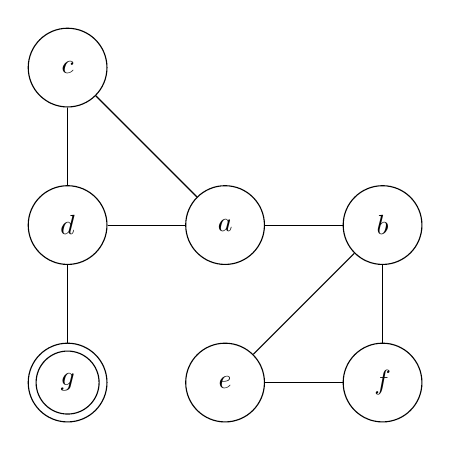
\begin{tikzpicture}
        % MDP i
        \node [draw, circle, minimum size=1cm] (a) at (2, 2) {$a$};
        \node [draw, circle, minimum size=1cm] (b) at (4, 2) {$b$};
        \node [draw, circle, minimum size=1cm] (c) at (0, 4) {$c$};
        \node [draw, circle, minimum size=1cm] (d) at (0, 2) {$d$};
        \node [draw, circle, minimum size=1cm] (e) at (2, 0) {$e$};
        \node [draw, circle, minimum size=1cm] (f) at (4, 0) {$f$};
        \node [draw, circle, minimum size=1cm] (g) at (0, 0) {$g$};
        \node [draw, circle, minimum size=0.8cm] at (0, 0) {};

        \draw[-] (a) -- (b);
        \draw[-] (a) -- (c);
        \draw[-] (a) -- (d);
        \draw[-] (b) -- (e);
        \draw[-] (b) -- (f);
        \draw[-] (c) -- (d);
        \draw[-] (d) -- (g);
        \draw[-] (e) -- (f);
        \draw[-] (d) -- (g);
    \end{tikzpicture}
    \caption{状態空間問題の例。エージェントはスタート地点$a$からゴール地点$g$を目指す。\\
    問題は\cite{edelkamp:2010:hst:1875144}より。
    }
	\label{fig:ssp-graph}
    % TODO: なんか面白そうにする
\end{figure}


\begin{figure}
	\centering
    \begin{tikzpicture}
        % MDP i
        \node (a0) at (4, 6) {$a$};

        \node (b1) at (2, 4) {$b$};
        \node (c1) at (4, 4) {$c$};
        \node (d1) at (6, 4) {$d$};

        \node (e2) at (0, 2) {$e$};
        \node (f2) at (2, 2) {$f$};
        \node (d2) at (4, 2) {$d$};
        \node (c2) at (6, 2) {$c$};
        \node (g2) at (8, 2) {$g$};

        \node (f3) at (0, 0) {$f$};
        \node (e3) at (2, 0) {$e$};
        \node (a31) at (3, 0) {$a$};
        \node (c3) at (4, 0) {$c$};
        \node (g3) at (5, 0) {$g$};
        \node (a32) at (6, 0) {$a$};

        \draw[-] (a0) -- (b1);
        \draw[-] (a0) -- (c1);
        \draw[-] (a0) -- (d1);
        \draw[-] (b1) -- (e2);
        \draw[-] (b1) -- (f2);
        \draw[-] (c1) -- (d2);
        \draw[-] (d1) -- (g2);
        \draw[-] (d1) -- (c2);
        \draw[-] (e2) -- (f3);
        \draw[-] (f2) -- (e3);
        \draw[-] (d2) -- (a31);
        \draw[-] (d2) -- (c3);
        \draw[-] (d2) -- (g3);
        \draw[-] (c2) -- (a32);
    \end{tikzpicture}
    \caption{状態空間問題の経路木。エージェントはスタート地点$a$からゴール地点$g$を目指す。\\
    }
    \label{fig:ssp-tree}
\end{figure}

%\captionlistentry[todo]{状態空間問題の例示}

この本では主に初期状態とゴール条件が与えられたとき、ゴール条件を満たすための経路を返す問題を探索する手法を考える。
特に本書の主眼は\ref{ch:state-space-problem}章から\ref{ch:heuristic-serach-variants}章までで扱う\define{状態空間問題}{state-space problem}である。


\ddef{ユニットコスト状態空間問題、state-space problem}{
	ユニットコスト状態空間問題$P = (S, A, s, T)$は状態の集合$S$、初期状態$s \in S$、ゴール集合$T \in S$、アクション集合$A = {a_1, ....,a_n}$、$a_i : S \rightarrow S$が与えられ、初期状態$s$からゴール状態へ遷移させるアクションの列を返す問題である。
}

よって、ユニットコスト状態空間問題はグラフにモデルすることで考えやすくなる。
ユニットコスト状態空間問題を表す\define{状態空間グラフ}{state-space graph}は以下のように定義される。

\ddef{状態空間グラフ、State-space graph}{
問題グラフ$G = (V, E, s, T)$は状態空間問題$P = (S, A, s, T)$に対して以下のように定義される。ノード集合 $V = S$、初期ノード$s \in S$、ゴールノード集合$T$、エッジ集合$E\subseteq V \times V$。エッジ$u,v\in E$は$a(u) = v$となる$a\in A$が存在する場合に存在し、そしてその場合にのみ存在する(iff)。
}

状態空間問題の\define{解}{solution}は以下の定義である。

\ddef{解、Solution}{
解$\pi = (a_1,a_2...,a_k)$はアクション$a_i \in A$の(順序付)配列であり、初期状態$s$からゴール状態$t \in T$へ遷移させる。すなわち、$u_i \in S$,$i \in \{0,1,...,k\}$, $u_0 = s, u_k = t$が存在し、$u_i = a_i(u_{i-1})$となる。
}

どのような解を見つけたいかは問題に依存する。
多くの問題では\define{経路コスト}{path cost}の合計を小さくすることを目的とする。

%すなわち、アクションに対してコストが定義されており、経路

\ddef{状態空間問題、Weighted state-space problem}{
	状態空間問題$P = (S, A, s, T, w)$はユニットコスト状態空間問題の定義に加え、コスト関数$w: A \rightarrow \mathbb{R}$がある。経路$(a_1,...,a_k)$のコストは$\sum^k_{i=1}w(a_i)$と定義される。
}

%ある解が可能なすべての解の中でコストが最小である場合、その解を最適解(optimal cost solution)であると言う。
本書ではこの状態空間問題を主に扱う。
状態空間問題のうちコストが定数関数である場合がユニットコスト状態空間問題である。
状態空間問題は重み付き(コスト付き)グラフとしてモデルすることが出来る。すなわち、$G = (V, E, s, T, w)$は状態空間グラフの定義に加え、エッジの重み$w: E \leftarrow \mathbb{R}$を持つ。

\ref{ch:blind-search}章で詳解するが、探索アルゴリズムは状態空間グラフのノード・エッジ全てを保持する必要はない。
全てのノード・エッジを保持した状態空間グラフを特に\define{明示的状態空間グラフ}{explicit state-space graph}と呼ぶとする。このようなグラフは、例えば隣接行列を用いて表すことが出来る。隣接行列$M$は行と列の大きさが$|V|$である正方行列であり、エッジ$(v_i, v_j)$が存在するならば$M_{i,j}=1$、なければ$M_{i,j}=0$とする行列である。
このような表現方法の問題点は行列の大きさが$|V|^2$であるため、大きな状態空間を保持することが出来ないことである。
例えば、\ref{sec:search-problem}節で紹介する15-puzzleは状態の数が$|V|=15!/2$であるため、隣接行列を保持することは現在のコンピュータでは非常に困難である。

そこで、探索アルゴリズムは多くの場合初期ノードとノード展開関数による\define{非明示的状態空間グラフ}{implicit state-space graph}で表せられる。

\ddef{非明示的状態空間グラフ、Implicit state-space graph}{
	非明示的状態空間グラフは初期状態$s \in V$、ゴール条件Goal: $V \rightarrow B = \{false, true\}$、ノード展開関数Expand: $V \rightarrow 2^V$によって与えられる。
}

探索の開始時、エージェントは初期ノードのみを保持する。エージェントは保持しているノードに対してExpandを適用することによって、新しいノードとエッジをグラフに加える。これを求める解を見つけるまで繰り返す。
Expandはある状態からの次の状態の集合を返す関数である。Expand関数は明示的に与えられるのではなく、ルールによって与えられることが多い。例えば将棋であれば、将棋のルールによって定められる合法手によって得られる次の状態の集合がExpand関数によって得られる。
これによって、エージェントは解を見つけるまでのノード・エッジだけ保持して必要な解を見つけることが出来る。


%\begin{example}

%\end{example}

%大まかには、情報なし探索による非明示的グラフは明示的グラフよりも指数的に小さく、ヒューリスティック探索による非明示的グラフは情報なし探索による非明示的グラフよりも更に指数的に小さいことが多い。

\begin{comment}
\section{状態空間問題の定式化}
\label{sec:search-problem-formulation}

状態空間問題の定式化の方法は様々である。
前述のように、状態空間$S$のすべての状態$s \in S$が陽に列挙されていることはあまりない。
多くの場合、状態は変数の列によって表せられる: $s = (v_0, v_1,...,v_n)$。これらの変数は状態変数と呼ぶこととする。これによって変数の組み合わせが状態空間となりグラフのノードを構成する。
そしてグラフのエッジはノード展開関数を用いて定義される。


\begin{table}
\caption{状態空間問題における問題の定式化。もっとも情報が多く与えられる定式化がドメイン依存エージェントであり、ヒューリスティック関数なども与えられる。ドメイン非依存エージェントはPDDLなどのモデル言語で書かれた入力が与えられ、その情報から用いるヒューリスティック関数や効率化手法を自動的に選択する必要がある。ブラックボックスエージェントは事前に何も与えられない、最も挑戦的な定式化である。}
\label{tbl:search-problem-formulation}
%\begin{adjustbox}{width=\textwidth}
\begin{tabular}{c|ccc}
	問題		& 状態遷移関数 	& ヒューリスティック関数 & 効率化 \\ \hline
	ドメイン依存 & Fully Available & hard-code & hard-code \\
	ドメイン非依存 (PDDL) & Fully Available & 自動生成する必要がある & ドメイン非依存の最適化・ポートフォリオ戦略 \\
	ブラックボックス & Unavailable (simulator) & Unavailable & 非許容的なノード・エッジの枝刈り
\end{tabular}
%\end{adjustbox}
\end{table}

% TODO: アルゴリズムを表にする?
\end{comment}


\section{状態空間問題の例}
\label{sec:search-problem}

状態空間問題の例をいくつか紹介する。
これらの問題はすべてヒューリスティック探索研究でベンチマークとして広く使われているものである。

%グリッド経路探索問題など、応用がありつつ、かつ分かりやすい問題を選んだ。
%グラフ探索アルゴリズムによって効率的に解くことが出来ると知られているドメインをいくつか紹介する。
%ここで詳解する問題はグラフ探索以外の手法でも解くことが出来る。


\subsection{グリッド経路探索 (Grid Path-finding)}
%\captionlistentry[todo]{Grid Pathfinding: なんかいい感じの絵}
%{\TODO Grid Pathfinding: なんかいい感じの絵}


\define{グリッド経路探索問題}{grid path-finding problem}は$k$(多くの場合$k=2$)次元のグリッド上で初期配置からゴール位置までの経路を求める問題である\cite{yap2002grid}。グリッドには障害物がおかれ、通れない箇所がある。エージェントが移動できる方向は4方向($A= \{up, down, left, right\}$)か8方向(4方向に加えて斜め移動)とする場合が多い。自由方向(Any Angle)の問題を扱う研究も存在する\cite{nash2007theta}。

\begin{figure}
	\includegraphics[width=0.5\textwidth]{figures/grid-pathfinding.png}
	\caption{グリッド経路探索問題}
	\label{fig:grid-pathfinding}
\end{figure}


Web上に簡単に試せるデモがあるので、参照されたい\footnote{\url{http://qiao.github.io/PathFinding.js/visual/}}。この本の画像の一部はこのデモをもとに作成している。この本で説明する様々なグラフ探索手法をグリッド経路探索に試すことが出来る。

グリッド経路探索はロボットのモーションプランニングやゲームAIなどで応用される\cite{algfoor2015comprehensive}。ストラテジーゲームなどでユニット(エージェント)を動かすために使われる \cite{cui2011based}。よく使われるベンチマーク問題集にもStarcraftのゲームのマップが含まれている\cite{sturtevant2012benchmarks}.
またグリッドは様々な問題を経路探索に帰着して解くことができるという意味でも重要である。例えば多重整列問題 (Multiple Sequence Alignment)はグリッド経路探索に帰着して解くことが出来る(後述)。
ロボットのモーションプランニングも経路探索に帰着することが出来る \cite{barraquand91}。すなわち、$k$個の関節の角度を変えて、現在状態からゴール状態へ遷移させたい。各関節の角度がグリッドの各次元に相当する。ロボットの物理的な構造により、関節のある角度の組み合わせは不可能である。不可能な組み合わせが、障害物の置かれたグリッドに相当する。よって、障害物を避けた経路というのが関節の動かし方ということになる。

%Starcraft 1ではA*探索が使われていた。
%しかしマルチエージェント
%マルチエージェント経路探索の場合はflocking / swarm AIが使われている。Starcraft 2では


\subsection{スライディングタイル (Sliding-tile Puzzle)}

多くの一人ゲームはグラフ探索問題に帰着することが出来る。スライディングタイルはその例であり、ヒューリスティック探索研究においてメジャーなベンチマーク問題でもある (図\ref{fig:15-puzzle}) \cite{johnson1879notes}。
$1$から$(n^2)-1$までの数字が振られたタイルが$n\times n$の正方形に並べられている。正方形には一つだけ{\it ブランク}と呼ばれるタイルのない位置があり、四方に隣り合うタイルのいずれかをその位置に移動する(スライドする)ことが出来る。スライディングタイル問題は、与えられた初期状態からスライドを繰り返し、ゴール状態にたどり着く経路を求める問題である。

\begin{figure}
\centering
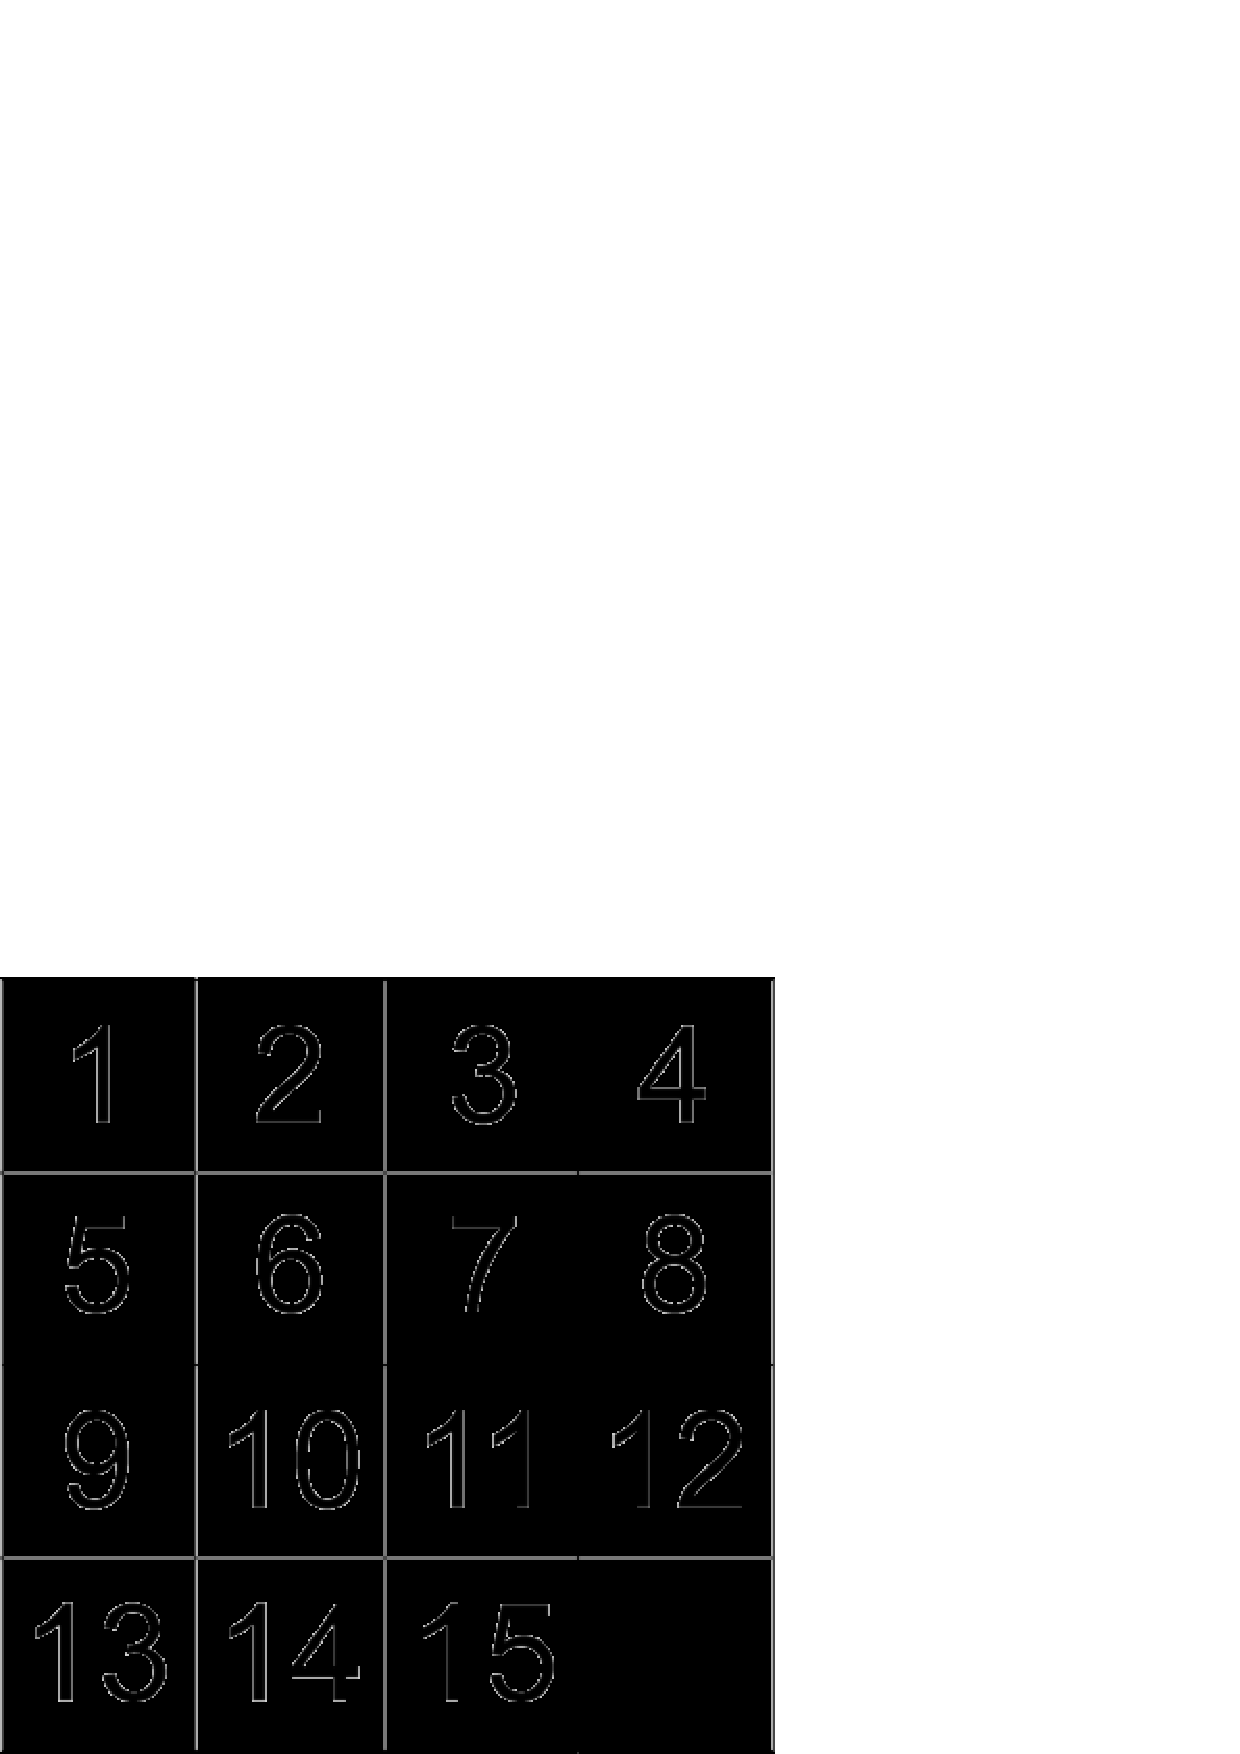
\includegraphics[bb=0 0 372 373,width=0.5\textwidth]{figures/15-puzzle.png}
\caption{15パズルのゴール状態の例}
\label{fig:15-puzzle}
\end{figure}


スライディングタイルの到達可能な状態の数は$|V| = (n^2)!/2$\footnote{スライディングタイルは偶奇性があり、到達不可能な状態がある\cite{johnson1879notes}。}であり、$n$に対して指数的に増加する。
可能なアクションは$A= \{up, down, left, right\}$の4つであり、アクションにかかるコストはすべて同じとする。

後述するが、ヒューリスティック探索のためには状態からゴール状態までの距離(コスト)の下界(lower bound)が計算できると有用である。
スライディングタイルにおける下界の求め方として最もシンプルなものは{\it マンハッタン距離ヒューリスティック}である。マンハッタン距離ヒューリスティックは各タイルの現在状態の位置とゴール状態の位置のマンハッタン距離の総和を取る。可能なアクションはすべて一つしかタイルを動かさないので、一回のアクションでマンハッタン距離は最大で1しか縮まらない。よって、マンハッタン距離はゴールまでの距離の下界である。

%ちなみに、スライディングタイルはpermutation problemの一つである。

\subsection{多重整列問題 (Multiple Sequence Alignment)}
\label{sec:msa}
生物学・進化学では遺伝子配列・アミノ酸配列の編集距離(edit distance)を比較することでニ個体がどれだけ親しいかを推定することが広く研究されている。
\define{多重整列問題}{Multiple Sequence Alignment} (MSA)は複数の遺伝子・アミノ酸配列が与えられた時、それらの配列間の編集距離とその時出来上がった配列を求める問題である。
2つの配列に対してそれぞれコストの定義された編集操作を繰り返し、同一の配列に並べ替える手続きをアライメントと呼ぶ。
2つの配列の編集距離は編集操作の合計コストの最小値である。
3つ以上の配列における距離の定義は様々考えられるが、ここでは全ての配列のペアの編集距離の総和を用いる。

MSAにおける可能な編集操作は置換と挿入である。置換は配列のある要素(DNAかアミノ酸)を別の要素に入れ替える操作であり、挿入は配列のある位置に要素を挿入する操作である。例えば(ABC, BCB, CB)の3つの配列のアライメントを考える。図\ref{fig:msa-cost}は置換と編集に対するコストの例である。-は欠損、すなわち挿入操作が行われたことを示す。アミノ酸配列における有名なコスト表としてPAM250\cite{pearson1990}があるが、ここでは簡単のため仮のコスト表を用いる。
図\ref{fig:msa-solution}はこのコスト表を用いたアライメントの例である。
このとき、例えば配列ABC-と-BCBの編集距離は(A,-)、 (B,B)、 (C,C)、 (-,B)のコストの総和であるので、図\ref{fig:msa-cost}を参照し、$5+0+1+5=11$である。(-BCB, --CB)の距離は$6$, (--CB, ABC-)の距離は$16$であるので、3配列の編集距離は$11+6+16=33$である。

$n$配列のMSAは$n$次元のグリッドの経路探索問題に帰着することが出来る\cite{korf:2000}。
図\ref{fig:msa-to-grid}は(ABC)と(BCB)の2つの配列による問題を表す。
状態$s$は2つの変数によって表現される:$(x_0, x_1)$。$x_0$は配列0のどの位置までアライメントを完了したかを表す変数であり、配列$i$の長さを$l_i$とすると定義域は$0 \leq x_0 \leq l_0$である。
全てのアライメントが完了した状態$s=(l_0, l_1)$がゴール状態である。
可能なアクションは$a=(b_0, b_1), (b_i=0, 1)$の形を取り、これは配列$i$に対して欠損を挿入する場合に$b_i=0$となる。
状態$s$に対してアクション$a$を適用した後の状態$s'$は$s'=(x_0+b_0, x_1+b_1)$となる。例えば図\ref{fig:msa-to-grid}は初期状態$s=(0,0)$に対して$a=(1,0)$を適用している。これは(A), (-)までアライメントを進めた状態に対応する。次に$a=(1,1)$が適用され、アライメントは(A,B), (-,B)という状態に至る。

このようにして、MSAはグリッド経路探索問題に帰着し、グラフ探索アルゴリズムよって解くことが出来る。
状態空間問題として考えた場合にMSAの難しさはアクションのコストが幅広いことにある。また、可能なアクションの数も配列の数$n$に対して$2^n-1$と大きい。

MSAは生物学研究に役立つというモチベーションから非常に熱心に研究されており、様々な定式化による解法が知られている。
詳しくは\cite{waterman1995introduction,
gusfield1997algorithms,edgar2006multiple}を参照されたい。


\begin{figure}
\centering
\includegraphics[width=0.95\textwidth]{figures/msa.png}
\caption{多重整列問題: 画像はwikipediaより。}
\label{fig:msa-gif}
\end{figure}


\begin{figure}
\centering
\subfloat[MSAの解の例]{
\begin{tabular}{ccccc}
	A & B & C & - \\
	- & B & C & B \\
	- & - & C & B \\
\end{tabular}
\label{fig:msa-solution}
} \hspace{4pt}
\subfloat[操作コスト表の例]{
\begin{tabular}{c|cccc}
	  & A & B & C & - \\ \hline
	A & 0 & 1 & 2 & 5 \\
	B &   & 0 & 3 & 5 \\
	C &   &   & 1 & 5 \\
	- &   &   &   & 0 \\	
\end{tabular}
\label{fig:msa-cost}
} \hspace{4pt}
\subfloat[グリッド経路探索への帰着]{
\begin{tabular}{c|cccc}
	  &   & A & B & C \\ \hline
	  & $\rightarrow$ & $\searrow$ &   &   \\
	B &   &   & $\searrow$ &   \\
	C &   &   &   & $\downarrow$ \\
	B &   &   &   & $\searrow$ \\
\end{tabular}
\label{fig:msa-to-grid}
}
\subfloat[グリッド経路探索への帰着]{
\begin{tabular}{c|cccc}
	  & A & B & C & - \\ \hline
	  & - & B & C & B \\ \hline
\end{tabular}
\label{fig:msa-to-grid-align}
}
\end{figure}


\subsection{倉庫番 (Sokoban)}
倉庫番(Sokoban)はAtariなどでパズルゲームであり、倉庫の荷物を押していくことで指定された位置に置くというゲームである。現在でも様々なゲームの中で親しまれている \cite{junghanns1997sokoban,culberson1997sokoban}。
プレイヤーは「荷物の後ろに回って押す」ことしか出来ず、引っ張ったり、横から動かしたりすることが出来ない。また、荷物の上を通ることも出来ない。
PSPACE-completeであることが知られている\cite{culberson1997sokoban}。

\begin{figure}
\centering
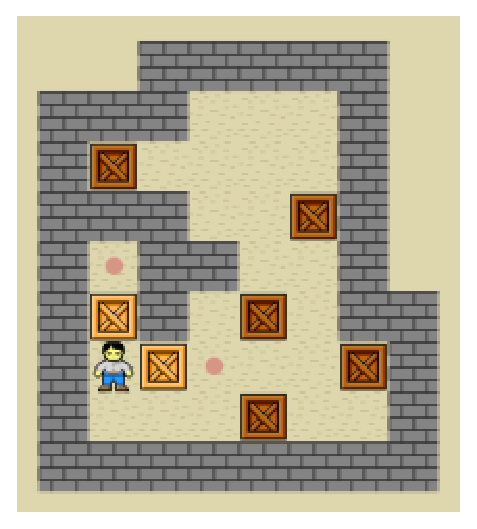
\includegraphics[bb=0 0 213 238,width=0.6\textwidth]{figures/sokoban.eps}
\caption{Sokoban: 画像はwikipediaより。}
\label{fig:sokoban}
\end{figure}

状態の表現方法は2通りあり、一つはグリッドの各位置に何が置いてあるかを変数とする方法である。もうひとつはプレイヤー、各荷物の位置に対してそれぞれ変数を割り当てる方法である。
可能なアクションは{\tt move-up}, {\tt move-left}, {\tt move-down}, {\tt move-right}, {\tt push-up}, {\tt push-left}, {\tt push-down}, {\tt push-right} の8通りである。{\tt move-*}はプレイヤーが動くアクションに対応し、コストは0である。{\tt push-*}は荷物を押すアクションであり、正のアクションコストが割当てられている。よって、倉庫番はなるべく荷物を押す回数を少なくして荷物を目的の位置に動かすことが目的となる。

グラフ探索問題として倉庫番を考えるときに重要であるのは、倉庫番は{\it 不可逆な}アクション(irreversible)があることである。
グリッド経路探索やスライディングタイルは{\it 可逆な} (reversible)問題である。
全てのアクション$a \in A$に対して$a^{-1} \in A$が存在し、$a(a^{-1}(s)) = s$かつ$a^{-1}(a(s)) = s$となる場合、問題は可逆であると言う。
可逆な問題は対応するアクションのコストが同じであれば無向グラフとしてモデルすることも出来、初期状態から到達できる状態は、すべて初期状態に戻ることが出来る。
一方、不可逆な問題ではこれが保証されず、詰み(trap)状態に陥る可能性がある (\ref{sec:difficulity}節)。

倉庫番では荷物を押すことは出来ても引っ張ることが出来ないため、不可逆な問題である。例えば、荷物を部屋の隅に置いてしまうと戻すことが出来ないため、詰み状態に陥る可能性がある問題である。
このような性質を持つ問題では特にグラフ探索による先読みが効果的である。

もうひとつ重要な問題は\define{ゼロコストアクション}{zero-cost action}の存在である。ゼロコストアクションはコストが0のアクションである。%TODO
倉庫番のアクションのうち{\tt move-up}, {\tt move-left}, {\tt move-down}, {\tt move-right}はコストゼロ($w(e)=0$)のアクションである。ヘタなアルゴリズムを実行すると無限に無駄なアクションを繰り返し続けるということもありうるだろう。


%倉庫の中には荷物がおかれ、エージェント(プレイヤー)は迷路を動き回り、
%このゲームで面白い/難しいのは、「荷物の後ろに回って押す」ことしか出来ず、引っ張ったり、横から動かしたりすることが出来ないという点である。

\subsection{巡回セールスパーソン問題 (Traveling Salesperson Problem, TSP)}

セールスパーソンはいくつかの都市に回って営業を行わなければならない。都市間の距離(=コスト)は事前に与えられている。
TSPは全ての都市を最短距離で回ってはじめの都市に戻る経路を求める、という問題である\cite{applegate2006traveling}。

\begin{figure}
\centering
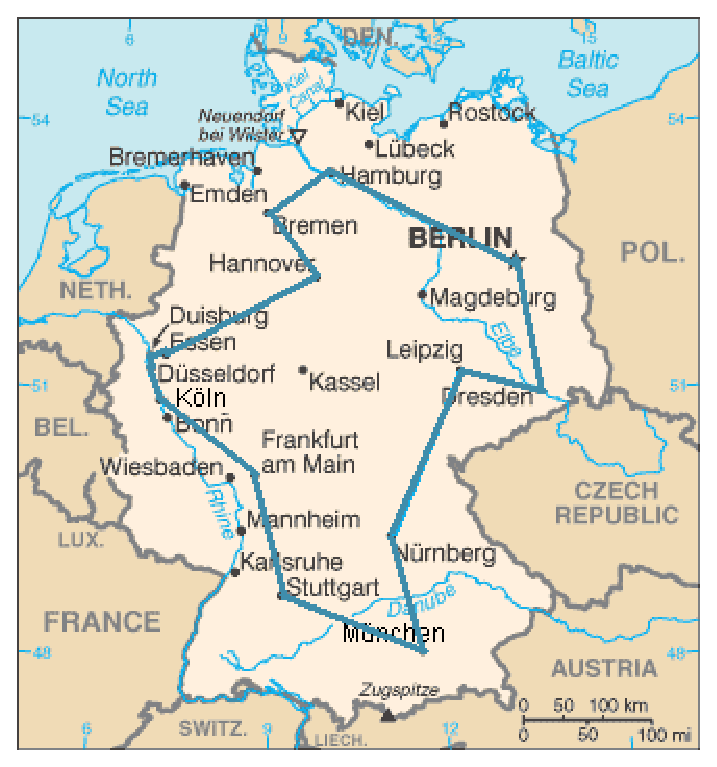
\includegraphics[bb=0 0 328 352,width=0.6\textwidth]{figures/tsp.eps}%TODO
\caption{巡回セールスパーソン問題: 画像はwikipediaより。}
\label{fig:sokoban}
\end{figure}

$n$個の都市があるとすると(最適・非最適含む)解の数は$(n-1)!/2$個である。
可能なアクションは「都市$i \in \{1..n\}$を訪れる」であり、一度訪れた都市には行けない。
TSPのゴール条件はすべての都市を訪れることである。よって、$n$回どれかアクションを実行すれば、とりあえず解を得ることが出来る。一方、最適解を得る問題はNP完全であることが知られている。

TSPの解の下界としては{\it 最小全域木} (minimum spanning tree)のコストがよく用いられる\cite{kruskal1956shortest,held1970traveling}。
グラフの{\it 全域木} (spanning tree)は全てのノードを含むループを含まない部分グラフである。
最小全域木は全域木のうち最もエッジコストの総和が小さいものである。
未訪問の都市によるグラフの最小全域木はTSPの下界となることが知られている。

TSPはヒューリスティック探索に限らず、様々なアプローチで研究されている問題ドメインである\cite{applegate2006traveling}。TSPについて特に詳しく知りたい方はそちらの教科書を参照されたい。


%\subsection{ペネトレーションテスト}

%\subsection{モデル検査}


\section{問題の性質・難しさ}
\label{sec:difficulity}
% TODO: どこにこの章を置くべきか?
% この節は最初に読む際は飛ばすべきである。

本書で定義した状態空間問題は小さなモデルである。
完全情報であり、状態遷移は決定論的である。
% 最小コスト経路探索は
それでもNP困難問題であり、難しい問題は難しい。
この節は問題の難しさがどのような要素に左右されるかを列挙する。

\begin{enumerate}
\item {\bf 状態空間の大きさ}

状態空間の大きさ$|S|$は大きい程概して問題は難しくなる。
特に状態空間が無限である場合深さ優先探索などのアルゴリズムは停止しない場合がある。
例えば状態変数に実数が含まれる場合、状態空間の大きさは無限になる。
% 状態空間の大きさがそのまま問題の難しさに直結するわけではない。

\item {\bf 分枝度}

ある状態$s$の\define{分枝度}{branching factor}はそのノードの子ノードの数を指す。
特に状態空間問題の分枝度は、すべての状態の分枝度の平均を指す。ただし多くの場合平均を厳密に求めることはなく、おおよその平均を指して分枝度をすることが多い。
分枝度が大きいほど問題は難しいとは限らない。
分枝度が多いほどグラフが密である、つまりエッジの数が多いことに対応する。
%エッジが多い程解の候補となる経路が多くなる。
分枝度を$b$とすると、あるノード$s$の子ノードの数は$b$個であり、孫ノードの数は$b^2$である。$s$からの深さ$d$のノードは$b^d$個である。

\item {\bf デッドエンド}

問題によってはある状態に到達するともう問題を解くことは出来ないというシチュエーションがある。例えば倉庫番は荷物を角においてしまうともう動かすことができない。これによってもう問題がクリアできなくなるということがある。このような問題では状態空間を広く探索し、デッドエンド状態のみを探索し続けるということをうまく避ける必要がある。例えば\ref{sec:greedy-best-first-search}節の貪欲最良優先探索はデッドエンドに入ってしまうとなかなか抜け出せないかもしれない。
% あるいはデッドエンドを検知する手法も考えられる。
概してデッドエンドがある問題では状態空間を広く探索する手法、探索済みの状態を記録する手法が有利であり、局所探索手法はうまくいかないことがある。
%このような問題では局所探索アルゴリズムではうまくいかないことがある。局所探索アルゴリズムは

\item {\bf 解の存在}

当然解が存在しない問題もありうる。
そのような場合、アルゴリズムは解が存在しないと示せれば理想的である。
一部のアルゴリズムは解が存在しない場合永遠に停止しない場合がある。
そのため解が存在しないことを検出するアルゴリズムの研究もされている \cite{backstrom2013fast,hoffmann2014distance}。

\end{enumerate}

\section{関連文献}

本章で定義した状態空間問題は基本となる定義であり、完全情報であり状態遷移が決定論的であることを仮定した。
状態遷移が決定論的ではなく確率的であると仮定したモデルは\define{マルコフ過程問題}{Markov Decision Process Problem} (MDP)と呼ばれている。
状態空間問題はMDPの特殊な場合である。
%図\ref{fig:mdp}のようにマルコフ過程問題もグラフによってモデルすることができる。
%グラフのノードは2種類あり、状態を表すノードと状態とアクションのペアを表すノードがある。
%状態とアクションのペアを表すノードからは可能な遷移先へのエッジが伸びている。また、このエッジには遷移確率のラベルがついている。
MDPは\define{強化学習}{reinforcement learning}における問題モデルとしても広く使われている。
MDPにおけるプランニング問題を解くためにはグラフ探索アルゴリズムも使えるが、動的計画法も用いられる \cite{Puterman}。
MDPからさらに不完全情報問題に拡張したものを\define{部分観測マルコフ過程問題}{partially observable Markov decision process problem} (POMDP)と呼ぶ。
POMDPにおけるプランニング問題の厳密解はBelief spaceプランニング \cite{POMDP, Kaelbling}によって求められるが、多くの場合計算困難(intractable)であるので近似手法が用いられる。

%状態遷移が他のエージェントによるアクションによって左右される問題をマルチエージェント問題と呼ぶ。特に将棋、囲碁やチェスなどの敵対二人ゲームはグラフ探索が活躍するドメインである。

本書では状態空間問題の解をゴールに到達するまでの経路と定義した。
状態空間問題のもう一つの定式化として、状態とアクションの組に対して\define{報酬}{reward} ($R: (S, A) \rightarrow \mathbb{R}$)を定義し、報酬を最大化する経路を求める問題がある。この定式化は特に強化学習で用いられる。

%状態空間問題の例としては\define{モデル検査}{model checking}がある。
%モデル検査はXXXYYY

%%%%%%%%%%%%%%%%%%%%%%%%%%%%%%%%%%%%%%%%%%%%%%%%%
%%% CHAPTER: Blind Search
%%%%%%%%%%%%%%%%%%%%%%%%%%%%%%%%%%%%%%%%%%%%%%%%%
\chapter{情報なし探索 (Blind Search)}
\label{ch:blind-search}

\ref{ch:introduction}章では様々な状態空間問題を紹介したが、それぞれの問題の解法はどれも沢山研究されている。
一つの指針としては、ある問題に特化した解法を研究することでその問題をより高速に解くというモチベーションがある。
これは例えばMSAのように重要なアプリケーションがある問題の場合に特に熱心に研究されることが多い。
一方、なるべく広い範囲の問題に対して適用可能な手法を研究するというモチベーションもある。
特に人工知能の文脈において、なるべく問題の知識を必要とせず、最小限の仮定のみを必要とする解法が求められる。
%ただしこのような手法はドメインに特化したプログラムと比べてパフォーマンスに劣ることが多い。

\ref{ch:introduction}章で紹介した状態空間問題を広く扱うことの出来る手法としてグラフ探索アルゴリズムがある。
本章では最もシンプルな問題(ドメイン)の知識を利用しない探索を紹介する。
情報なし探索 (Blind Search)は状態空間グラフのみに注目し、背景にある問題に関する知識を一切使わないアルゴリズムである。
このような探索では{\bf 1. 重複検知を行うか 2. ノードの展開順序}が重要になる。
重複検出は訪問済みの状態を保存しておくことで同じ状態を繰り返し探索することを防ぐ手法である。対価としては、メモリの消費量が非常に大きくなることにある。
ノードの展開順序とは、例えば幅優先探索・深さ優先探索などのバリエーションを指す。
効率的な展開順序は問題によって大きく異なり、問題を選べばこれらの手法によって十分に効率的な探索を行うことが出来る。
これらの探索手法は競技プログラミングでもよく解法として使われる\cite{skiena2006programming}。また、いわゆるコーディング面接でもグラフ探索アルゴリズムは頻出である\cite{mcdowell2011cracking}。
%\ref{ch:search-performance}章はグラフ探索の高速化の紹介をするので、特に競技プログラミングに興味がある場合はそちらも参照されたい。% TODO
情報なし探索は\cite{cormen01}の22章Elementary Graph Algorithmsにも詳しく説明されている。

\begin{comment}
\begin{table}
\caption{木探索とグラフ探索}
\label{tbl:tree-vs-graph-search}
%\begin{adjustbox}{width=\textwidth}
\caption{木探索とグラフ探索の違い。状態の重複検出を行わない手法を木探索と呼ぶ。探索する状態空間が木であるか否かは関係しない。グラフ探索は重複検出を行うことで同じ状態を複数回無駄に探索することを防ぐ。重複検出のためには生成済みノードをすべて保存するデータ構造クローズドリストが必要になる。}
\begin{tabular}{c|ccc}
				& 重複検出  	  & 保存するノード & 完全性 \\
	木探索  		& 重複検出しない & オープンリストのみ & ループを含むグラフである場合停止性を満たさない \\
	グラフ探索 		& 重複検出する  & オープンリストとクローズドリスト & (状態空間が有限ならば)完全 \\ 
\end{tabular}
%\end{adjustbox}
\end{table}


\begin{table}
\label{tbl:basic-priority}
%\begin{adjustbox}{width=\textwidth}
\caption{ノードの展開順序。}
\begin{tabular}{c|cc}
	展開順序  	& プライオリティ 	& 性質 \\  
	幅優先	& $\arg \min_n d(n)$ & ユニットコストドメインだと最初に発見した解が最適解である \\
	深さ優先 	& $\arg \max_n d(n)$ & メモリ消費が少ない場合がある \\
	最良優先	& $\arg \min_n g(n)$ & 非負コストドメインで最適解が得られる \\
\end{tabular}
%\end{adjustbox}
\end{table}
\end{comment}


\section{木探索アルゴリズム (Tree Search Algorithm)}
\label{sec:tree-search-algorithm}
木探索アルゴリズムはグラフ探索アルゴリズムの基礎となるフレームワークであり、本文で紹介する手法のほとんどがこのフレームワークを基礎としているといえる。
アルゴリズム\ref{alg:implicit-tree-search}は木探索の疑似コードである。

\begin{algorithm}[tbh]
\caption{木探索 (Implicit Tree Search)}
\label{alg:implicit-tree-search}
	\Input{initial node $s$, weight function $w$, successor generation function $Expand$, goal function $Goal$}
	\Output{Path from $s$ to a goal node $t \in T$, or $\emptyset$ if no such path exists}
	$Open \leftarrow \{s\}$\;
	\While{$Open \neq \emptyset$} {
		$u \leftarrow Open.pop()$\;
		\If {$Goal(u)$} {
			\Return $Path(u)$\;
		}
		$Succ(u) \leftarrow Expand(u)$\;
		\For {each $v \in Succ(u)$} {
			$Open.insert(v)$\;
			$parent(v) \leftarrow u$\;
		}
 	}
	\Return $\emptyset$\;
\end{algorithm}

\begin{algorithm}[tbh]
\caption{Expand}
\label{alg:expand}
	\Input{Parent node $s$, a set of actions applicable to the state $A(s)$}
	\Output{A set of child nodes $S$}
	\For {$a \in A(s)$} {
		$s' \leftarrow a(s)$\;
		$d(s') \leftarrow d(s) + 1$\;
		$g(s') \leftarrow g(s) + w(s, s')$\;
		$S \leftarrow S \cup {s'}$\;
	}
	\Return $S$\;
\end{algorithm}


以下、(k)と書いて疑似コードのk行目を指すことにする。
木探索はオープンリスト\footnote{歴史的な経緯でリストと呼ばれているが、データ構造がリストで実装されるという意味ではない。効率的なデータ構造は\ref{ch:search-performance}章で紹介する。}と呼ばれるノードの集合をPriority queueに保持する。探索の開始時には、初期状態のみがオープンリストに入っている(1)。
木探索は、このオープンリストから一つノード$u$を選び(3)、ゴール条件を満たしているかを確認する(4)。満たしていれば初期状態から$u$への経路を返す。満たしていなければ、そのノードを展開する(6-)。展開とは、そのノードの子ノードを列挙し、オープンリストに入れる(8)ことを指す。

アルゴリズム\ref{alg:expand}は展開関数の動作を表している。
初期状態からノード$n$への最小ステップ数を深さ$d$と呼び、最小経路コストを$g$値と呼ぶ。すべてのアクションのコストが1のドメインであれば任意の$n$に対して$d(n) = g(n)$が成り立つ。
状態を更新すると同時に$g$値を更新する。これによって解を発見した時に解ノードの$g$値が解のコストとなる。
なお、状態$s$に対して適用可能なアクションの集合$A(s)$は与えられていると仮定する。

探索の進行によってエージェントが保持する情報は変化していく。ここでは探索がどのように進行するかを記述するため、以下の3つの言葉を定義する:

\begin{enumerate}
\item 展開済みノード: $Expand$によって子ノードが参照されたノードを指す。$Open$からは取り除かれたノードである。
\item 生成済みノード: $Open.insert$によって$Open$に一度でも入れられたノードを指す。
\item 未生成ノード: 状態空間内のまだ生成されていないノード。よって、非明示的グラフに保持されていない。
\end{enumerate}

非明示的グラフ木探索の強みは、生成済みノードのうち展開済みではないもののみを$Open$に保持すればよいことにある。未生成ノード、展開済みノードはメモリ上に保持する必要がない。
一方、これの問題は、一度展開したノードが再び現れた場合、{\bf 再展開 (reexpansion)}をすることになる。よって、グラフがより木から遠いほど(複数の経路で到達可能なノードがあるほど)同じノードを何度も再展開することになり、効率が悪くなってしまう。もっと言えば、木探索アルゴリズムは状態数が有限であっても停止しない場合がある。
これらが問題になるような問題ドメインである場合は後述する重複検出を使うグラフ探索 (\ref{sec:graph-search-algorithm}節)を使うと良いだろう。

{\bf 紛らわしいが、木探索アルゴリズムはグラフを探索するアルゴリズムである。}
グラフ探索アルゴリズムのうち、重複検出を行わない手法を木探索アルゴリズムと呼ぶ。
疑似コードでは明示されていないが、オープンリストはプライオリティキューであり、どの順番でノードを取り出すかを決めなければならない ($Open.pop$の実装にあたる)。
探索アルゴリズムの性能はこのプライオリティの設定方法に強く依存する。
本章の\ref{sec:breadth-first-search}節以降、及び\ref{ch:heuristic-search}章はこのプライオリティをどうデザインするかについて議論をする。

%同じ状態を複数回展開すると計算資源を無駄にすることになるのでなるべく重複を避けたい。


%木探索ベースのアルゴリズムの問題は、解が存在しない場合に停止性を満たさないことである。よって、この手法は解が間違いなく存在することが分かっている問題に対して適用される。あるいは、解が存在することを判定してから用いる。


\section{グラフ探索アルゴリズム (Graph Search Algorithm)}
\label{sec:graph-search-algorithm}


明示的グラフのあるノードが初期状態から複数の経路でたどり着ける場合、同じ状態を表すノードが木探索による非明示的グラフに複数現れるということが生じる。このようなノードを\define{重複}{duplicate}と呼ぶ。ノードの重複は計算資源を消費してしまうので、効率的な\define{重複検出}{duplicate detection}の方法は重要な研究分野である。

{\bf 本書ではノードの重複検出を行う探索アルゴリズムを狭義にグラフ探索アルゴリズムと呼び、重複検出を行わない探索を木探索と区別する。}

%ノードの重複の確認にはいくつかメリットがある。一つは、停止性を満たすことである。すなわち、最悪グラフのノードをすべて展開して停止する。もう一つは、

\begin{algorithm}[tbh]
\caption{グラフ探索 (Implicit Graph Search)}
\label{alg:implicit-graph-search}
	\Input{Implicit problem graph with initial node $s$, weight function $w$, successor generation function $Expand$, goal function $Goal$}
	\Output{Path from $s$ to a goal node $t \in T$, or $\emptyset$ if no such path exists}
	$Closed \leftarrow \emptyset$\;
	$Open \leftarrow \{s\}$\;
	\While{$Open \neq \emptyset$} {
		$u \leftarrow Open.pop()$\;
		\If {$Goal(u)$} {
			\Return $Path(u)$\;
		}
		$Succ(u) \leftarrow Expand(u)$\;
		\For {each $v \in Succ(u)$} {
			\If{$Closed.find(v.state) is null$} {
				$Open.insert(v)$\;
				$parent(v) \leftarrow u$\;
				$Closed.insert(u)$\;
			}
			\Else {
				$v' \leftarrow Closed.find(v.state)$\;
				\If {$v.g < v'.g$} {
					$Open.insert(v)$\;
					$parent(v) \leftarrow u$\;
					$Closed.insert(v)$\;

					$Open.remove(v')$\;
					$Closed.remove(v')$\;
				}
			}
		}
 	}
	\Return $\emptyset$\;
\end{algorithm}


重複検出のためには生成されたノードを\define{クローズドリスト}{closed list}に保存する。一度クローズドリストに入れられたノードはずっとクローズドリストに保持される。
ノード展開関数から子ノードが生成されたら、その子ノードと同じ状態を保持するノードがクローズドリストに存在するかを確認する。
もし存在しなければ、そのノードは重複ではない。なのでそのノードをオープンリストに加える。
存在した場合の処理は少しややこしい。
新たに生成されたノード$n$の$g$値のほうが先に生成されクローズドリストにあるノード$n'$の$g$値よりも小さい場合が存在する。このとき、$n$をそのまま捨ててしまうと、そのノードの$g$値が本来の値よりも大きく評価されてしまう。

$g$値をそのノードに到達できる既知の最小コストにするためには、まずクローズドリストに保存されているノードの$g$値を$g(n')$から$g(n)$に更新しなければならない。
加えて、ノード$n$を\define{再展開}{reexpansion}しなければならない。
ノード$n$の子ノード$c$は$n'$の子ノードとして展開されていたわけであるが、そのとき$g(c) = g(n') + w(n', c)$として計算された。この値は$g(c) = g(n) + w(n, c)$に更新しなければならない。$w(n', c) = w(n, c)$なので、$g(n') - g(n)$だけ$g$値が小さくなる。なので、$c$の子ノードも再展開をする必要がある。そしてそのまた子ノードも。。。というように、再展開が生じるとそこから先のノードをすべて再展開する必要がある。これはかなり大きなコストになることが多いので、可能な限り避けたい処理である。

%なので常に$g$値をそのノードに到達できる既知の最小コストに更新する。

重複が存在した場合に必ずノードを捨てることができる場合も存在する。
まず、解の最適性が必要でない場合$g$値を更新する必要はない。$g$値が過大に評価されても解経路は解経路のままであり、ただ解経路のコストが大きくなるだけである。
また、例えば幅優先探索では探索の過程で生成されるノードの$d$値は単調増加する。もしユニットコストドメインならば$g$値も単調増加である。つまりノード$n$と重複したノード$n'$がクローズドリストにあったとすると、$g(n) \geq g(n')$が成立する。この場合、解最適性を保ったまま$n$を安全に捨てることができる。
また、状態空間グラフが木である場合は重複が発生しない。
なお、後述するA*探索\ref{sec:astar-search}ではある条件を満たせば再展開は行わずに解の最適性が満たせることが知られている。これがA*探索がstate-of-the-artとして重要視されている理由である。

ここで「ノード」と「状態」の言葉の使い分けに注意したい。
状態とは状態空間問題における状態$s$である。ノードは状態$s$を含み、$f$値、$g$値の情報を含む。
重複検出を行わない木探索の場合、同じ状態を保持するノードが2つ以上存在しうる。
重複検知は同じ状態を保持するノードをマージする処理に相当する。この処理を行うと同じノードに複数の経路で到達するようになり、グラフは木ではなくなる。

% 重複検出を行ってもノードの再展開が必要になる場合は存在するが、ほとんどの場合重複検出を行わない場合よりもはるかに再展開の回数は少なくなる。
% 実行時間で見ると重複検出を行ったほうがほぼ確実に効率的である。
重複検出の問題はメモリの使用量である。重複検出を行うためには生成済みノードをすべてクローズドリストに保存しなければならない。なので展開済みノードの数に比例した空間が必要になる。
クローズドリストの効率的な実装については\ref{sec:closed-list}節で議論をする。

なお、重複検出はノードが生成されたときではなく、ノードが展開されるときに遅らせることができる。
オープンリストには重複したノードが含まれることになるが、ノードの展開時には重複をチェックするので重複したノードの展開は防げる、ということである。これは\define{遅延重複検出}{delayed duplicate detection}と呼ばれ、\ref{sec:delayed-duplicate-detection}節で議論をする。



\section{幅優先探索 (Breadth-First Search)}
\label{sec:breadth-first-search}

探索のパフォーマンスにおいて重要になるのは{\bf どのようにして次に展開するノードを選択するか}にある($Open.pop()$)。
ヒューリスティック探索の研究の非常に大きな部分はここに費やされているといえる。
シンプルかつ強力なノード選択方法はFirst-in-first-out (FIFO)である。あるいは幅優先探索と呼ぶ。

幅優先探索の手順は非常に単純であり、FIFOの順に$Open$から取り出せばいいだけである。
これをもう少し大きな視点で、{\it どのようなノードを優先して探索しているのか}を考えてみたい。
初期状態から現在状態にたどり着くまでの経路の長さをノードの$d$値と定義する。
すると、幅優先探索の$Open.pop()$はアルゴリズム\ref{alg:brfs-open}のように書くことが出来る。
ユニットコスト問題である場合、$d$値は$g$値と一致する。

幅優先探索のメリットは初めに発見した解が最短経路長であることである。
問題がユニットコストドメインであれば、最短経路が最小コスト経路であるので、最適解が得られる。
なお、後述するBest First Searchと区別するため、Breadth-First Searchの略称はBrFSを用いることがある (Best First SearchはBFSとなる)。

\begin{algorithm}
\caption{Breadth-First Search: $Open.pop()$}
\label{alg:brfs-open}
	\Output{Node $n$}
	\Return $\arg \min_{n \in Open} d(n)$
\end{algorithm}

重複検出を用いた幅優先探索で図\ref{fig:ssp-graph}の問題を解こうとすると、オープンリスト、クローズドリストの中身は表\ref{tbl:brfs-traj}のように遷移する。

\begin{table}[tbh]
\centering
\caption{重複検出を用いた幅優先グラフ探索のオープンリスト・クローズドリスト (\cite{edelkamp:2010:hst:1875144}より)}
\begin{tabular}{c|c|l|l|l}
	ステップ & ノードの選択 & オープンリスト & クローズドリスト & \\
	1 	  & \{\}       & \{a\}      & \{\} \\
	2     & a        & \{b,c,d\}  & \{a\} \\
	3     & b        & \{c,d,e,f\} & \{a,b\} \\
	4     & c        & \{d,e,f\}   & \{a,b,c\} \\
	5     & d        & \{e,f,g\}   & \{a,b,c,d\} \\
	6     & e        & \{f,g\}     & \{a,b,c,d,e\} \\
	7     & f        & \{g\}       & \{a,b,c,d,e,f\} \\
	8     & g        & \{\}        & \{a,b,c,d,e,f,g\} & ゴールを発見 \\
\end{tabular}
\label{tbl:brfs-traj}
\end{table}

\section{深さ優先探索 (Depth-First Search)}
\label{sec:depth-first-search}

幅優先探索が幅を優先するのに対して深さ優先探索はもっとも深いノードを優先して探索する。

深さ優先探索は解がある一定の深さにあることが既知である場合に有効である。
例えばTSPは全ての街を回ったときのみが解であるので、街の数が$n$であれば全ての解の経路長が$n$である。
このような問題を幅優先探索で解こうとすると、解は最も深いところにしかないので、最後の最後まで解が一つも得られないということになる。一方、深さ優先探索なら$n$回目の展開で一つ目の解を見つけることが出来る。
表\ref{tbl:dfs-traj}は図\ref{fig:ssp-graph}の問題で重複検出ありの深さ優先探索を行った場合のオープンリスト・クローズドリストの遷移を示した。図\ref{fig:ssp-tree}と合わせてノードが展開される順序を確認すると良い。

良い解、最適解を見つけたい場合でも深さ優先探索が有用である場合がある。
早めに一つ解が見つけられると、その解よりも質が悪い解にしかつながらないノードを\define{枝刈り}{pruning}することが出来る。ノード$n$を枝刈りするとは、ノード$n$をオープンリストに加えずそのまま捨てることを指す。つまりアルゴリズム\ref{alg:implicit-tree-search}における$Open.insert(v)$をスキップする。詳しくは\ref{sec:pruning}章で解説する。

% TODO: Frequent Itemset Mining

\begin{algorithm}[tbh]
\caption{Depth-First Search: $Open.pop()$}
\label{alg:dfs-open}
	\Output{Node $n$}
	\Return $\arg \max_{n \in Open} g(n)$
\end{algorithm}

\begin{table}[tbh]
\centering
\caption{重複検出を用いた深さ優先グラフ探索のオープンリスト・クローズドリスト (\cite{edelkamp:2010:hst:1875144}より)}
\begin{tabular}{c|c|l|l|l}
	ステップ & ノードの選択 & オープンリスト   & クローズドリスト & \\
	1 	  & \{\}     & \{a\}       & \{\} \\
	2     & a        & \{b,c,d\}   & \{a\} \\
	3     & b        & \{e,f,c,d\} & \{a,b\} \\
	4     & e        & \{f,c,d\}   & \{a,b,e\} \\
	5     & f        & \{c,d\}     & \{a,b,e,f\} \\
	6     & c        & \{d\}       & \{a,b,e,f,c\} \\
	7     & d        & \{g\}       & \{a,b,e,f,c,d\} \\
	8     & g        & \{\}        & \{a,b,e,f,c,d,g\} & ゴールを発見 \\
\end{tabular}
\label{tbl:dfs-traj}
\end{table}

\subsection{再帰による深さ優先探索}
\label{sec:recursive-depth-first-search}

上述の実装はオープンリストを利用した深さ優先探索である。
一般的にアルゴリズム \ref{alg:implicit-tree-search}、\ref{alg:dfs-open}に従った方法の実装は効率的ではない \footnote{深さ優先探索を並列化する場合はオープンリストを用いる場合がある}。
深さ優先探索は再帰によって効率的に実装することができる (アルゴリズム \ref{alg:recursive-dfs})。
ここでこのアルゴリズムにはオープンリストがないことに注目したい。
これは実装が簡単というだけではなく、消費メモリが少なく、実行時間が少ないというメリットがある。

\begin{algorithm}[tbh]
\caption{Depth-First Search (DFS)}
\label{alg:recursive-dfs}
	\Input{Node $s$, weight function $w$, successor generation function $Expand$, goal function $Goal$}
	\Output{Path from $s$ to a goal node $t \in T$, or $\emptyset$ if no such path exists}
	\If {$Goal(s)$} {
		\Return $s$\;
	}
	$Succ(u) \leftarrow Expand(u)$\;
	\For {each $v \in Succ(u)$} {
		\If {$DFS(v) \neq \emptyset$} {
			\Return $(s, DFS(v))$
		}
	}
	\Return $\emptyset$\;
\end{algorithm}


\section{ダイクストラ法 (Dijkstra Algorithm)}
\label{sec:dijkstra}

\define{ダイクストラ法}{Dijkstra's Algorithm}はグラフ探索アルゴリズムの一種であり、グラフ理論の教科書な
どでも登場する情報科学全体に多岐に渡り重要とされるアルゴリズムである \cite{dijkstra1959note}。
例えばネットワークルーティングにおけるlink state algorithmなどにDijkstraが使われる\cite{mcquillan1980new}。
%初期状態からノード$n$への既知の最小経路コストを$g$値と呼び、$g(n)$と書く。
ダイクストラ法はグラフ探索において$g$値が最も小さいノードを優先して展開するアルゴリズムと説明することができる。
つまりグラフ探索の疑似コード\ref{alg:implicit-graph-search}の$Open.pop$を以下のように実装すればダイクストラ法である。

\begin{algorithm}[tbh]
\caption{Best-First Search: $Open.pop()$}
\label{alg:dfs-open}
	\Output{Node $n$}
	\Return $\arg \max_{n \in Open} g(n)$
\end{algorithm}

{\bf 深さ優先探索との違いは重複検出を行うところである。}
ダイクストラ法は非負コストグラフにおいて最短経路を返す。
ユニットコストドメインでは$\forall n (g(n) = d(n))$であるため、幅優先探索と同じ動作をする。
フィボナッチヒープ \cite{fredman1987fibonacci}を用いてオープンリストを実装したダイクストラ法は$O(|E| + |V|log|V|)$時間でであることが知られている\cite{fredman1987fibonacci}。%任意の非負コスト有向グラフにおける最短経路問題を解くアルゴリズムとして知られている中で最も
%Bellman-Fordアルゴリズムも重要である。
そのため、後述するヒューリスティック関数が得られない問題においてはとりあえずダイクストラ法を試してみることは有効である。


% \section{上手く行かない場合}

% データ構造を確認する(\ref{ch:search-performance}章)

% ヒューリスティック関数が使えるか否か(\ref{ch:heuristic-search}章)


\section{関連文献}

ダイクストラ法はコストが負のエッジを持つ場合にうまくいかない。
負のエッジを含む問題を解くための手法としてはベルマン-フォード法が有名である \cite{bellman1958routing,ford1956network}。

%状態遷移が確率的である場合(マルコフ過程問題)や敵対二人ゲームの場合は、AND/OR木による探索アルゴリズムが使われる。
%\define{動的計画法}{dynamic programming}やモンテカルロ木探索などの手法が用いられる \cite{bellman2013dynamic}。

ダイクストラ法などの情報なし探索は\define{組み合わせ最適化}{combinatorial optimization}の手法として使われることも多い\cite{tarjan1983data}。

\subsection{No Free Lunchとヒューリスティック}

No Free Lunch定理 \cite{Wolpert and Macready}はコンピュータサイエンスの多くの最適化問題で言及される定理である。
状態空間問題におけるNo Free Lunch定理の主張は以下である。
\begin{theorem}
すべての可能なコスト関数による状態空間問題の集合を考える。
この問題集合に対する平均性能はすべての探索アルゴリズムで同じである。
\end{theorem}

問題に対して知っている知識を利用して効率化をすることができる。
すなわち、ある問題集合への性能を犠牲に、ある問題集合への性能を向上させることができる。
与えられている問題の特徴を知っていれば、その問題に対する性能の良いアルゴリズムを選ぶことができる。
それが次章で扱うヒューリスティック探索の行うことである。

\chapter{ヒューリスティック探索 (Heuristic Search)}
\label{ch:heuristic-search}

\ref{ch:blind-search}章では問題の知識を利用しないグラフ探索手法について解説した。
本章では問題の知識を利用することでより効率的なグラフ探索を行う手法、特にヒューリスティック探索について解説する。

\section{ヒューリスティックとは?}
\label{sec:heursitic}

経路探索問題を幅優先探索で解くことを考えよう。
図\ref{fig:grid}の初期状態からゴールへの最短経路の長さはXである。このとき、幅優先探索は図\ref{fig:grid-brfs}の領域を探索する。
しかし人間が経路探索を行うときにこんなに広い領域を探索しないだろう。なぜか。
それは人間が問題の特徴を利用して、このノードを探索したほうがよいだろう、という推論を働かせているからである。
問題の特徴を利用してノードの{\bf 有望さ}を\define{ヒューリスティック関数}{heuristic function}として定量化し、ヒューリスティック関数を利用した探索アルゴリズムをヒューリスティック探索と呼ぶ。
ヒューリスティック関数は人間が自分の知識を利用してコーディングする場合もあるが、自動行動計画問題などでは自動的にヒューリスティックを生成する手法も広く使われている。


%\captionlistentry[todo]{ヒューリスティックとは: grid, grid-brfsの図を挿入}
%{\TODO ヒューリスティックとは: grid, grid-brfsの図を挿入}

\section{ヒューリスティック関数 (Heuristic Function)}
\label{sec:heuristic-function}
ヒューリスティック関数はある状態からゴールまでの最短距離の見積もりである \cite{hart68formal}。

\ddef{ヒューリスティック関数、heuristic function}{
	ヒューリスティック関数$h$はノードの評価関数である。$h: V \rightarrow \mathbb{R}_{\geq 0}$
}

ヒューリスティックの値が小さいノードほどゴールに近いと推測できるので、探索ではヒューリスティック値が小さいノードを優先して展開する。
ヒューリスティック関数の値をそのノードの$h$値と呼ぶことが多い。


ヒューリスティック関数の望ましい性質として、まず正確である方が望ましい。すなわち、$h$値が実際のゴールまでの最短距離に近いほど、有用な情報であると言える。
ノード$n$からゴールまでの正しい最短コストを$h^*$とする。
ヒューリスティック関数$h$が任意の$n$に対して$h(n) = h^*(n)$である場合、\define{完璧なヒューリスティック}{Perfect Heuristic}と呼ぶ。%完璧なヒューリスティック関数がある場合、A*探索は
反対に役に立たないヒューリスティック関数は$h(n) = 0$などの定数関数である。これはどのノードに対してもゴールまでの距離が同じだと推測しているということであり、つまり何も主張をしていない。このようなヒューリスティックをブラインドヒューリスティックと呼ばれる。ブラインドヒューリスティックを使った探索は、\ref{ch:blind-search}章で扱った情報なし探索の一種といえる。

現実には完璧なヒューリスティックはなかなか得られないが、多くの場合これに近いほど必要な展開ノード数が小さいことが知られている\cite{helmert:08}。

もう一つ望ましい性質は$h$値が最適解コストの下界である場合である。
\ref{sec:astar-search}章で解説するが、$h$値が最短距離の下界である場合、それを用いた効率的な探索アルゴリズム(A*探索、重み付きA*探索)において解コストに理論的保証が得られることが広く知られている。
$h$値が常に最適解コストの下界であるヒューリスティック関数を許容的なヒューリスティックと呼ぶ。

\ddef{許容的なヒューリスティック、admissible heuristic}{
	ヒューリスティック関数$h$は最適解のコストの下界である場合、許容的である。すなわち、全てのノード$u \in V$に対して$h(u) \leq h^*(u)$が成り立つ。
}

ただし、$h^*(u)$はノード$u$からゴールノード集合$T$のいずれかへたどり着くための最短経路である。%$h^*$はパーフェクトヒューリスティックと呼ぶ。

一般に、許容的なヒューリスティックを得る方法としては、元問題の{\bf 緩和問題}を解き、その最適解コストをヒューリスティック値とすることである。ある問題の緩和問題とは、解集合に元の問題の解を含む問題を指す。要するに元の問題より簡単な問題である\footnote{解が多いほど簡単であるとは一概には言えないが}。

%許容的よりも強い性質としてとして無矛盾性がある。
もう一つ重要な性質は無矛盾性である。

\ddef{無矛盾なヒューリスティック、consistent heuristic}{
	ヒューリスティック関数$h$は全てのエッジ$e = (u, v) \in E$に対して$h(u) \leq h(v) + w(u,v)$が成り立つ場合、無矛盾である。
}

無矛盾性は特に\ref{sec:astar-search}章で後述するA*探索において探索の効率性に重要な性質である。
また、無矛盾なヒューリスティックのうちゴールノードの$h$値が0となるヒューリスティックは許容的である。

\begin{theorem}
ゴールノード$n \in T$に対して$h(n) = 0$となる無矛盾なヒューリスティックは許容的なヒューリスティックである。
\end{theorem}

\begin{proof}

あるノード$n_0$からゴールノード$n_k \in T$への最短経路(ノードの列)を$(n_0, n_1,...)$と置く。無矛盾なヒューリスティック$h(n)$は
\begin{align}
	h(n_0) &\leq h(n_1) + w(n_0, n_1) \\
			&\leq h(n_2) + w(n_0, n_1) + w(n_1, n_2) \\
			&... \\
			&\leq h(n_k) + \sum_{i=0..k-1}(w(n_i,n_{i+1})) \\
			&= h^*(n_0)
\end{align}
よって$h(n_0) \leq h^*(n_0)$より許容的である。

\end{proof}

後述するA*探索においてこれら二つの性質は非常に有用である。
%無矛盾性の主張は、ヒューリスティックの値が小さいほどゴールに近いということを意味する。つまり、ノード$n_0, n_1$に対して$h(n_0) < h(n_1)$ならば、$n_0$からゴールへの最小コストは$n_1$からゴールへの最小コストよりも小さい。
%これのうれしい点は、次にどのアクションを選択するべきかを考える際、よりゴールに近いノードに向かったほうが良いだろう、と判断をすることができる点にある。
%例えばグリッド経路探索問題におけるマンハッタン距離ヒューリスティックは無矛盾なヒューリスティックである。マンハッタン距離ヒューリスティックは現在位置とゴール位置のマンハッタン距離を$h$値とする。


\section{A*探索 (A* Search)}
\label{sec:astar-search}

%\captionlistentry[todo]{ダイクストラ法の問題点を図示}
%{\TODO ダイクストラ法の問題点を図示}
ダイクストラ法は初期状態からそのノードまでのコストである$g$値が最小のノードを展開していく。これは間違った方針ではないだろうが、理想的にはゴール状態に向かっていくノードを展開していきたい。図\ref{fig:dijkstra-grid}はダイクストラ法による状態空間の探索を図示したものである。ダイクストラ法はゴールがどこにあるかということを無視して探索を進めているため、図のように探索空間が広がっていく。
%人間の目で見れば一目で右に探索していけばよいというのは分かる。そのような人間の持っている知識を利用して探索を効率化出来ないだろうか?

\define{A*探索}{A* search}はゴールまでの距離を見積もる\define{ヒューリスティック関数}{heuristic function}を用いることで図\ref{fig:astar-grid}のようにゴールに向かって探索していくことを目指した手法である。

A*探索はヒューリスティック探索の代名詞である、最も広く知られている
手法である\cite{fikes:71}。
A*探索は以下の$f$値が最小となるノードを優先したグラフ探索アルゴリズムである。

\begin{equation}
	f(n) = g(n) + h(n)
\end{equation}


ノード$n$の$f$値は、初期状態から$n$を通過してゴール状態に辿り着くためのコストの見積もりである。$g$値は初期状態からノード$n$までの既知の最短経路コストである。一方$h$値はヒューリスティック関数による$n$からゴール状態までの最短経路の見積もりである。
A*探索は非明示的グラフ探索アルゴリズム(アルゴリズム\ref{alg:implicit-graph-search})の一つであり、$Open.pop()$を$f$値最小ノードを返すようにしただけである \ref{alg:astar-search}。

\begin{algorithm}[tbh]
\caption{A* Search: $Open.pop()$}
\label{alg:astar-search}
	\Output{Node $n$}
	\Return $\arg \min_n g(n) + h(n)$
\end{algorithm}

$g(n)$のみでノードを選択するダイクストラ法(\ref{sec:dijkstra}章)と比較すると、A*探索はゴール状態までのコストの見積もりを考慮して次に展開するノードを決めている。

図\ref{fig:grid-astar-mdheuristic}は\define{マンハッタン距離ヒューリスティック}{Manhattan distance heuristic}によるA*探索である。
青いノードは展開済みノード、緑のノードはオープンリストに入れられた未展開ノードである。
ダイクストラ法による図\ref{fig:grid-dijkstra}と比較すると、展開済み・未展開ノードの数が少なく済んでいることがわかるだろう。


\begin{figure}[tbh]
\includegraphics[width=0.4\linewidth]{./figures/grid-astar-mdheuristic.png}
\caption{A*探索}
\label{fig:grid-astar-mdheuristic}
\end{figure}

\begin{figure}[tbh]
\includegraphics[width=0.4\linewidth]{./figures/grid-dijkstra.png}
\caption{ダイクストラ法}
\label{fig:grid-dijkstra}
\end{figure}

A*に用いるヒューリスティック関数は正確であるほど良いが、それに加えて許容的、無矛盾であるという性質も有用である。

\begin{theorem}
ヒューリスティックが許容的である時、A*は最適解を返す。
\end{theorem}
\begin{proof}

%全てのノードnは展開時にg(n)がnに辿り着くための最短経路コストの値である。%これは無矛盾性か
許容的なヒューリスティック$h(n)$は$n$からゴールへの経路の下界である。よって、ゴール状態の$h$値は$0$である。つまりゴール状態の$f$値は$g$値と同じである。この解の$g(n')$値を$f*$と置く(解のコストに相当)。
A*のノードの展開順に従うと、$f*$のノードを展開する前に全ての$f<f*$のノードが展開される。
これらのノードがいずれもゴール状態でなければ、$g(n) \leq f(n)$より、$g(n)<f*$となるゴール状態がない。すなわち、$f*$が最適解のコストとなり、$n'$がその時のゴール状態である。

\end{proof}

A*探索はノードの\define{再展開}{reexpansion}が生じる可能性がある。
{\TODO kobayashi et alのような図を}

無矛盾なヒューリスティックである場合、全てのノード$n$は展開時までに$g(n)$が$n$に辿り着くための最短経路コストの値になる。

\begin{theorem}
無矛盾なヒューリスティックを用いたA*探索はノードの再展開が生じない。
\end{theorem}

% TODO: exercise?
%\begin{proof}
%\end{proof}

\begin{theorem}
ゴールノードが存在するとする。
ゴールノード$n \in T$の深さ$d(n)$の中でもっとも小さいものを$d$とする ($d = min_{n \in T} (d(n))$)。
完璧なヒューリスティックを用いたA*探索は$d$回のノードの展開でゴールを発見し停止する。
\end{theorem}

\begin{proof}
\end{proof}



効率的なA*探索を実装するために考えるべきことはいくつかある。
まずヒューリスティック関数の正確さはパフォーマンスに大きな影響を与える。
テーブル\ref{tbl:heuristic-comparison}は15パズルにおいてブラインドヒューリスティック、マンハッタン距離ヒューリスティック、パターンデータベースヒューリスティック(後述)を用いたA*の性能比較である。
{\bf 論文を探す}

\begin{table}[tbh]
\caption{15パズルにおけるヒューリスティックの性能の比較}
\label{tbl:heuristic-comparison}
\end{table}

\subsection{重み付きA*探索 (Weighted A*)}
\label{sec:weighted-astar-search}

許容的なヒューリスティックを用いたA*探索は最適解が得られるが、必ずしも最適解がほしいわけではない場合もある。解のクオリティよりもとにかく解が何か欲しい、という場合もある。
最適解ではない解を\define{非最適解}{suboptimal solution}と呼び、最適解に限らず解を発見するアルゴリズムを\define{非最適探索}{suboptimal search}、あるいは\define{局所探索}{local search}と呼ぶ。
\define{重み付きA*探索}{weighted A*} (wA*)は解のクオリティが落ちる代わりにより素早く買いにたどり着くための手法である \cite{wilt2010comparison}。
wA*は重み付き$f$値、$f_w$が最小のノードを優先して探索する。

\begin{equation}
	f_w(n) = g(n) + w h(n)
\end{equation}

\begin{algorithm}
\caption{Weighted A*: $Open.pop()$}
\label{alg:wastar-open}
	\Output{Node $u$}
	\Return $\arg \min_{n \in Open} f_w(n)$
\end{algorithm}


\begin{theorem}
許容的なヒューリスティックを用いた重み付きA*探索は最適解のコスト$f^*$に対して、発見される解のコストが$w f^*$以下であることを保証する。
\end{theorem}
%\captionlistentry[todo]{wA*: 解コストの上界の証明}
{\TODO wA*: 解コストの上界の証明}
%\begin{proof}
%\end{proof}

wA*の利点はA*よりもはるかに高速であることである。
多くの場合、$w$の大きさに対して指数的な高速化が期待できる。これは深さ$d$のノードの個数は$d$に対して指数的(分枝度を$b$とすると$b^d$個)であることに対応する。

wA*などの非最適探索を使う場合は最適解が得られないので、許容的でないヒューリスティックと組み合わせて使われることが多い。許容的でないアルゴリズムはその代わりに高速であることがある。% TODO lama?

wA*の解は最適解のコストの上界になるので、A*探索の枝刈りに用いることが出来る。
A*探索を実行する前にwA*を走らせ、解の上界$c^*$を得、A*探索実行時にノード$n$に対して$f$値が$f(n) \geq c^*$である場合、そのノードを枝刈りする。このテクニックは多重配列アライメントなどに使われる\cite{ikeda1999enhanced}。

図\ref{fig:grid-wastar}はA*とwA*の比較である (ここではエージェントは4方向に動けるとする)。
wA*の重み$w$は5としている。
wA*の展開・生成ノード数がA*よりも少ないことがわかるだろう。
その一方wA*で発見された解がA*で発見された解よりも遠回りなことがわかる。

\begin{figure}
\includegraphics[width=0.3\linewidth]{./figures/grid-astar.png}
\includegraphics[width=0.3\linewidth]{./figures/grid-wastar-5.png}
\includegraphics[width=0.3\linewidth]{./figures/grid-gbfs.png}
\caption{A*, wA*, GBFS比較}
\label{fig:grid-wastar}
\end{figure}

\subsection{貪欲最良優先探索 (Greedy Best-First Search)}
\label{sec:greedy-best-first-search}

wA*の例で見たように、$g$値に対して$h$値に重きを置くことによって解のクオリティを犠牲により高速に解を得ることができる。
問題によっては解のクオリティはあまり重要でなかったり、そもそもクオリティという概念がないことがある。
このようにとにかく解があればよいという場合は\define{貪欲最良優先探索}{Greedy Best-First Search}が使われることが多い \cite{wilt2010comparison}。

\begin{algorithm}
\caption{Greedy Best-First Search: $Open.pop()$}
\label{alg:gfs-open}
	\Output{Node $u$}
	\Return $\arg \min_n h(n)$
\end{algorithm}

貪欲最良優先探索は$g$値を無視し、$h$値のみで展開順を決定する。つまりwA*の$w$を無限大にしたものである。

貪欲最良優先探索は解のクオリティに保証がない。
しかし多くの問題で高速に解を発見できるとても強力な手法である。

図\ref{fig:grid-wastar}は貪欲最良優先探索である。wA*よりもさらに生成ノード数が少ないことが分かるだろう。


\section{ヒューリスティック関数の例}
\label{sec:heuristic-example}

\ref{sec:heuristic-function}章にあるように、なるべく正確であり、許容的、無矛盾なヒューリスティックが望ましい。
一般に、許容的なヒューリスティックを得る方法としては、元問題の{\bf 緩和問題}を解き、その最適解コストをヒューリスティック値とすることである。ある問題の緩和問題とは、解集合に元の問題の解を含む問題を指す。要するに元の問題より簡単な問題である\footnote{解が多いほど簡単であるとは一概には言えないが}。
グラフ探索アルゴリズムにおいて緩和問題を作る方法は様々あるが、一つはグラフのエッジを増やすことで緩和が出来る。グラフのエッジを増やすには、問題の可能なアクションを増やすなどの方法がある。

\subsection{グリッド経路探索:マンハッタン距離}

4方向グリッド経路探索問題の元問題は障害物のあるグリッドに移動することは出来ない。グリッド経路探索で有効なヒューリスティックの一つはマンハッタン距離ヒューリスティックである。これは現在位置とゴール位置のマンハッタン距離を$h$値とする。マンハッタン距離の意味としては、障害物を無視した最短経路の距離であるので、グラフのエッジを増やした緩和問題である。
このように、問題の性質を理解していれば許容的なヒューリスティック関数を設計することが出来る。
8方向グリッドにおいても斜め方向を加えた距離を考えることで許容的なヒューリスティックとすることが出来る。Any angleグリッドならば直線距離が許容的なヒューリスティックである。

\begin{figure}[tbh]
\includegraphics[width=0.3\linewidth]{./figures/grid-manhattan.png}
\caption{グリッド経路探索におけるマンハッタン距離の例}
\label{fig:grid-manhattan}
\end{figure}

\subsection{スライディングタイル:マンハッタン距離}
スライディングタイルにおけるマンハッタン距離ヒューリスティックは各タイルの現在の位置とゴール状態の位置のマンハッタン距離の総和を$h$値とする。
スライディングタイル問題において一度に動かせるタイルは1つであり、その距離は1つである。
そのため、マンハッタン距離ヒューリスティックは許容的なヒューリスティックである。
% 無矛盾

\begin{figure}[tbh]
\includegraphics[width=0.3\linewidth]{./figures/tile-manhattan.png}
\caption{スライディングタイルにおけるマンハッタン距離の例}
\label{fig:tile-manhattan}
\end{figure}

%\subsection{MSA:ペア間距離和}

\subsection{巡回セールスパーソン問題:最小全域木}
TSPの解の下界としては{\it 最小全域木} (minimum spanning tree)のコストがよく用いられる。
グラフの{\it 全域木} (spanning tree)は全てのノードを含むループを含まない部分グラフである。
最小全域木は全域木のうち最もエッジコストの総和が小さいものである。
未訪問の都市によるグラフの最小全域木はTSPの下界となることが知られている。

\begin{figure}[tbh]
\includegraphics[width=0.3\linewidth]{./figures/tsp-mst.png}
\caption{巡回セールスパーソンにおける最小全域木}
\label{fig:tsp-mst}
\end{figure}


\section{上手く行かない場合}

ヒューリスティック探索が思ったより遅い場合考えるべきことはいくつかある。

まず考えるべきは、そもそもヒューリスティック探索によって解くべき問題なのかという点である。
制約プログラミングや他の組合せ最適化手法なら効率的な問題かもしれない。
似たような問題が他の手法によって解かれていないかを調べてみると良い。

ヒューリスティック探索が良さそうだと思ったら、試しにwA*にしてみて、weightを大きく取ってみよう。
おおまかに言うとwA*の実行速度はwの大きさに対して指数的に速くなる。w=1だと全く解けそうにない問題でもw=2にすると一瞬で解けることがある。
もしweightを10くらいにしてもすぐに解が発見できなければ、おそらくその問題で最適解を発見するのは非常に難しい。このような問題に対しては最適解を見つけることは諦め、局所探索 (\ref{ch:local-search}章)を使ったほうが良いだろう。
wA*でも解が見つけられない場合はそもそも解がない問題かもしれない。解がない場合は制約プログラミングのソルバーを使うと素早く検出できることが多い。

wA*で非最適解を見つけられる場合なら、工夫すればA*で最適解を見つけることができるかもしれない。
その場合まず、おおまかな探索空間の大きさを見積もり、そして1秒間に何ノードが展開されているかを確認すると良い。
ヒューリスティック探索の実行時間はおおまかには(展開するノード数)と(1ノードの展開にかかる時間)の積である。

%例えばA*探索はC++でスライディングタイル問題だと秒間XXXノードが展開できる。
もし秒間に展開されているノードの数が少ない場合、プロファイラを使ってどのオペレーションに時間がかかっているかを確認するべきだろう。多くの場合実行時間の大半をオープンリスト、クローズドリスト、ノードの展開関数(現在の状態とアクションから状態を計算する関数)のいずれかが占めている、ということがわかるだろう。

オープンリスト、クローズドリストの処理に時間がかかっている場合はデータ構造の改良によって問題が解決するかもしれない。効率的なデータ構造の設計については\ref{ch:search-performance}章を参照されたい。
あとはプロセスのメモリ消費量を確認してみよう。A*はメモリ消費も激しい。
実行時間が遅いのは、メモリを使いすぎていてメモリスワップが起きているからかもしれない。
より大きなメモリを使うか、IDA*などのメモリの消費量の少ない手法を試してみると良いかもしれない。

ノードの展開関数に時間がかかる場合はその実装を工夫するか、ノードの展開回数を最小限に抑えるしかない。
ノードの展開回数を減らす方法はなかなか難しいが、例えばヒューリスティック関数の改良によって可能である。
ほんの少しのヒューリスティック関数の改善によって探索の効率は劇的に上がりうる。
% 例えばスライディングタイル問題ではTODO。

これらの方法でもまだ解けない場合、扱っている問題は純粋なA*で解くには結構難しい問題かもしれない。
1968年にA*が初めて提案されてから、様々な発展手法が考案されてきた。
\ref{ch:heuristic-search-variants}章で紹介する最新の手法を試してみれば解けるかもしれない。


\section{関連文献}

\define{最良優先探索}{best-first search}という言葉は2種類の定義があることに注意したい。
\cite{todo}は最良優先探索をA*を含むアルゴリズムの集合を定義した\cite{todo}。
一方\cite{todo}はゴールに最も近い、つまり$h$値が一番小さいノードを常に最優先して展開するアルゴリズムを最良優先探索と呼んだ\cite{todo}。本書ではこの方法は貪欲最良優先探索と呼んでいる。


同じ問題に対して重み付きA*を繰り返し$w$値をだんだんと小さくしていくことでだんだんと解のクオリティを向上させることができる。
この方法をAnytime A*と呼ぶ \cite{}。


\chapter{自動行動計画問題 (Automated Planning Problem)}
%\chapter{古典的プランニング問題 (Classical Planning Problem)}
\label{ch:classical-planning}

本書の冒頭でグラフ探索アルゴリズムが人工知能のための技術として研究されていると説明した。
人工知能とはさまざまな定義で使われる言葉であるが、グラフ探索は自動推論や自動行動計画のために使うことができるために研究されている。
この章では人工知能の一分野である\define{自動行動計画問題}{automated planning problem}について説明する \cite{ghallab:04}。
自動行動計画は初期状態から命題集合で表される目的を達成するための{\bf プラン}を発見する問題である。
自動行動計画のためのモデルは様々提案されている。
最も基本となるモデルは古典的プランニング問題である \cite{fikes:71}。
古典的プランニングは完全情報\footnote{正確には完全情報ではなく、アクションの決定のために必要な情報がすべて得られるという風に定義される。例えば問題に全く関係ない冗長な変数が含まれる場合、その情報がエージェントに与えられない場合を考えることができる。このような問題も冗長な変数を無視し古典的プランニング問題で扱うことができる。}、決定的状態遷移を仮定とするモデルであり、状態空間問題に含まれる \cite{fikes:71}。
古典的プランニングによって様々な実問題を表すことができる。例えばロジスティック\cite{helmert2010scanalyzer,sousa2013toward}、セルアセンブリ\cite{asai2014fully}、遺伝子距離計算\cite{erdem2005genome}、ビデオゲーム\cite{lipovetzky2015a}など、様々な応用問題を含むモデルである。

完全情報、決定的状態遷移の仮定を緩和した問題(確率的モデルや不完全情報モデル)もグラフ探索によって解かれることが多いが、本文の範囲外とする。詳細は詳しい教科書を参照されたい\cite{russelln03}。
なお、プランニング問題はA*などの状態空間探索アルゴリズム以外にも、SATやCSPなどの制約充足問題に変換して解く方法もある \cite{ernst1997automatic,do2001planning}。古典的プランニングのための解法としてはグラフ探索アルゴリズムがstate-of-the-artであるが、例えばマルチエージェント経路探索問題などではSATに変換する手法が効率的であることが知られている \cite{sharon2015conflict}。
%本書は
%これらの面白い議論があるが、本書の範囲外とする\cite{kautz:92}。

\section{定義}
\label{sec:planning-definition}

古典的プランニングは述語論理によって世界が記述される\cite{fikes:71}。
Proposition $AP$は世界の状態において何が真・偽であるかを記述する。
世界の状態はエージェントがアクションを行うことによって遷移し、遷移後の状態は遷移前の状態と異なるpropositionが真・偽でありうる。
古典的プランニングの目的は与えられた初期状態からゴール条件を満たすまでのアクションの列を求めることにある。
以下、定義は\cite{edelkamp:2010:hst:1875144}に従う。

\begin{definition}[古典的プランニング問題、Classical Planning Problem]
古典的プランニング問題は有限状態空間問題$P = (S,A,s_0,T)$の一つである。
$S \subseteq 2^{AP}$は状態の集合であり、$s_0 \in S$は初期状態、$T \subseteq S$はゴール状態の集合、$A: S \rightarrow S$は可能なアクションの集合である。
\end{definition}

古典的プランニング問題の最も基本となるSTRIPSモデル\cite{fikes:71}の場合、ゴール条件は命題(proposition)のリストで表せられる$Goal \subseteq AP$。ゴール状態の集合$T$は$p \in Goal$となるすべての$p$が真である状態の集合である。
アクション$a \in A$は適用条件$pre(a)$、効果($add(a)$, $del(a)$)で表せられる。適用条件$pre(a) \subseteq AP$はアクション$a$を実行するために状態が満たすべきpropositionの集合である。効果$add(a)$はアクション$a$を適用後に真になるpropositionの集合であり、$del(a)$は偽になる集合である。
従って、アクション$a$を状態$s$に適用後の状態$s' = suc(s,a)$は
\begin{equation}
	s' = (s \cup add(a)) \setminus del(a)
\end{equation}
である。

このようにして、古典的プランニング問題は状態空間問題に帰着することが出来る。

状態空間問題はさらにグラフ探索問題に帰着することができる。
グラフ探索による解法の利点は任意の状態空間問題に対して解法となる点である。
例えば各ドメインに対して特化した手法を用いることも考えられるが、そのような人間の知識を必要とする手法を考えることは人工知能技術の目的とは離れてしまう。
グラフ探索によって古典的プランニング問題を解く場合、問題の定義のみが必要である。解法についての知識は必要ではない。
つまりプランナーを使う側に立ってみれば、何かの問題解決を行うにあたって問題の定義のみを与えれば、それをどうやって解くかを考えることなく、問題の解を得ることができるのである。
逆に言えば、効率的なグラフ探索アルゴリズムが開発できれば、あらゆる状態空間問題に対して適用できる汎用な手法が高速化できた、ということだ。

% TODO: show fast-downward.
fast-downward \cite{helmert2006}はプランニング問題を解くstate-of-the-artのプランナーである。
本書で紹介するアルゴリズムの多くがfast-downwardに組み込まれている。


%なのでグラフ探索アルゴリズムとプランニング研究の大きなテーマの一つとして、どのようにして少ない前提知識から効率的なグラフ探索を行うことができるかが盛んに研究されている。
%具体的には効率的なヒューリスティック関数を自動生成する研究や、並列探索などのハードウエアを利用した方法、あるいは洗練されたデータ構造を利用する方法などが

%As such, a classical planning problem can be solved by an A* search ($G(V', E', w'), s_0', T'$); $V' = S$, $e(v_i, v_j) \in E'$ exists if there exists $a$ such that $v_j = succ(v_i, a)$, $s_0' = s_0$, $T' = T$.

% TODO: PDDLの文字フォントを\textttに
\section{プランニングドメイン記述言語: Planning Domain Definition Language}
\label{sec:pddl}

Planning Domain Definition Language (PDDL) \cite{aeronautiques1998pddl}はプランニング問題を記述されるために用いられる言語の一つである。PDDLはプランニング問題を一階述語論理で表現する。
PDDLはドメイン記述とインスタンス記述の2つに分けられ、Lispのような文法で書かれる。
図\ref{fig:pddl-domain}と図\ref{fig:pddl-instance}はブロックスワールド問題のドメイン記述とインスタンス記述である。
ここでドメインとインスタンスは計算理論などで定義される\define{問題}{problem}と\define{インスタンス}{instance}に対応する。
ドメイン記述は問いの集合を定義し、インスタンスは一つの問いを指定する。
例えば「グリッド経路探索問題」はドメインであり、そのうちの特定の一つのマップがインスタンスに対応する。
ドメイン記述には\define{述語}{predicate} (\texttt{predicates})と\define{アクションスキーム}{action scheme} (\texttt{action})がある。
インスタンス記述には\define{オブジェクト}{object} (\texttt{objects})と初期状態(\texttt{init})、ゴール状態(\texttt{goal})がある。
これら以外にも例えばオブジェクトの型など様々な文法があるが、簡単のためここでは割愛する。
これらの記述によって古典的プランニング問題が定義される。

まず、命題集合$AP$は述語に含まれる変数にオブジェクトを割り当てることによって得られる。
図の例だと例えば\texttt{(on A B), (on A C), (ontable D),...}などの命題が$AP$に含まれる。

アクション集合$A$はアクションスキームに含まれる変数にオブジェクトを割り当てることによって得られ、アクションの変数は\texttt{parameters}に定義される。

アクション$a$の適用条件$pre(a)$はアクションスキームの\texttt{precondition}にオブジェクトを割り当てることで得られる。\texttt{effect}のうち\texttt{not}のついていない命題は$add(a)$に対応し、\texttt{not}のついた命題は$del(a)$に対応する。
例えばアクション\texttt{(pickup A)}の適用条件は{\texttt{(clear A), (ontable A), (handempty)}}、追加効果は{\texttt{(holding A)}}、削除効果{\texttt{(ontable A), (clear A), (handempty)}}である。
初期状態$s_0$は\texttt{init}の命題集合である。この例では{\texttt{(CLEAR C) (CLEAR A) (CLEAR B) (CLEAR D) (ONTABLE C) (ONTABLE A)}}である。
ゴール条件$Goal$は\texttt{goal}の命題集合である。つまり、ゴール状態集合$T$は$Goal$を含む状態の集合である。

PDDLのミソは一階述語論理によってプランニング問題を記述する点である。
状態空間に含まれる命題を一つ一つ記述するのではなく、述語とオブジェクトの組み合わせによって複数の命題をコンパクトに記述することができる。
また、インスタンス記述を変えることで同じドメインの異なるインスタンスをモデルすることができる。
例えばブロックスワールドのドメイン記述はそのままに、インスタンス記述のオブジェクトや\texttt{init}などを変えることで違う問いにすることができる。

PDDLは状態空間問題だけでなくより広く様々な問題を扱うことができる \cite{aeronautiques1998pddl,fox2003pddl2}。
fast downwardはPDDLの文法の多くをサポートしているので試してみるには便利である。

\begin{figure}
\includegraphics[width=0.8\linewidth]{./figures/blocks-image.png}
\caption{Blocks worldドメイン}
\label{fig:sliding-token}
\end{figure}

\begin{figure}
%\begin{adjustbox}{width=\textwidth,keepaspectratio}
\lstset{language=pddl,basicstyle=\ttfamily\footnotesize,breaklines=true}
\begin{lstlisting}
;;;;;;;;;;;;;;;;;;;;;;;;;;;;;;;;;;;;;;;;
;;; 4 Op-blocks world
;;;;;;;;;;;;;;;;;;;;;;;;;;;;;;;;;;;;;;;;
(define (domain BLOCKS)
  (:requirements :strips)
  (:predicates (on ?x ?y)
	       (ontable ?x)
	       (clear ?x)
	       (handempty)
	       (holding ?x)
	       )

  (:action pick-up
	     :parameters (?x)
	     :precondition (and (clear ?x) (ontable ?x) (handempty))
	     :effect
	     (and (not (ontable ?x))
		   (not (clear ?x))
		   (not (handempty))
		   (holding ?x)))

  (:action put-down
	     :parameters (?x)
	     :precondition (holding ?x)
	     :effect
	     (and (not (holding ?x))
		   (clear ?x)
		   (handempty)
		   (ontable ?x)))
  (:action stack
	     :parameters (?x ?y)
	     :precondition (and (holding ?x) (clear ?y))
	     :effect
	     (and (not (holding ?x))
		   (not (clear ?y))
		   (clear ?x)
		   (handempty)
		   (on ?x ?y)))
  (:action unstack
	     :parameters (?x ?y)
	     :precondition (and (on ?x ?y) (clear ?x) (handempty))
	     :effect
	     (and (holding ?x)
		   (clear ?y)
		   (not (clear ?x))
		   (not (handempty))
		   (not (on ?x ?y)))))
\end{lstlisting}
%\end{adjustbox}
\caption{blocks-worldのdomainファイル}
\label{fig:pddl-domain}
\end{figure}

\begin{figure}
%\begin{adjustbox}{width=\textwidth,keepaspectratio}
\lstset{language=pddl,basicstyle=\ttfamily\footnotesize,breaklines=true}
\begin{lstlisting}
(define (problem BLOCKS-3)
(:domain BLOCKS)
(:objects A B C)
(:INIT (CLEAR C) (CLEAR B) (ONTABLE C) (ONTABLE B)
 (ON C A) (HANDEMPTY))
(:goal (AND (ON A B) (ON B C)))
)

\end{lstlisting}
%\end{adjustbox}
\caption{blocks-worldのinstanceファイル}
\label{fig:pddl-instance}
\end{figure}

\section{古典的プランニング問題の例}
\label{sec:classical-planning-example}

プランニングは様々な問題解決に役立てることができる。
ここでは簡単にプランニングによってどのような問題がモデルされているかを紹介する。

\begin{enumerate}
\item エアポート (airport)
空港の地上の交通管理を行う問題である。
飛行機の離着陸の時間が与えられるのに対し、安全かつ飛行機の飛行時間を最小化する交通を求める問題である。

\item サテライト (sattellite)
人工衛星は与えられた現象を撮影し、地球にデータを送らなければならない。
このドメインはNASAの人工衛星の実際の応用から考案されたものである。

\item ローバー (rovers)
ローバーとは惑星探査ロボットのことである。
この問題は惑星探査ロボットのグループを使って惑星を探索する計画を作る問題である。
ロボットらは興味深い地形などの写真を取るなどの作業を実行する必要がある。
このドメインもNASAの応用をもとにしたものである。

\item パイプスワールド (pipesworld)
複数の原油の油田から複数の目的地にパイプを通して送りたい。
各目的地に定められた量を送るように調整することが目的である。
パイプのネットワークはグラフとしてモデルされており、また同時に原油を通せないパイプの組が存在する。

\item セルアセンブリ (cell assembly)
セルアセンブリは狭いセルの中で働き手が複雑な製品を作成する工場システムである。
大規模な製造ラインと比較して、
セルアセンブリは主に中程度の数(100個程度など)の製品を作るために使われる。
製品の開発や受注生産などに対応して、今生産しなければならない製品を手早く作成するためのセルの行動プランを考えることが問題の目的である。
\cite{asai2014}

\item ゲノムリアレンジメント (Genome rearrangement)
ゲノムリアレンジメントは多重整列問題の一つである。
ゲノム間の編集距離とは類似性を測るための指標として使われ、生物の進化の歴史をたどるために使われる。編集距離はあるゲノムから操作を繰り返してもう一方のゲノムに変換するためのコストの総和として定義される。
プランニングモデルを用いることでより様々な操作を定義することができる。例えば遺伝子の位置に入れ替えなど、\ref{sec:msa}節で説明したように単純にグリッド経路探索に落とし込むことのできない複雑な操作を考えることができる。
\cite{erdem2005}

\item トラック (trucks)
ロジスティクスと呼ばれる問題の一種である。
トラックを運転してすべての荷物をそれぞれ定められた運び先に届ける問題である。
ただしトラックが運べる荷物の総量は有限であるため、それを考慮して経路を考えなければならない。加えて、届けるまでの期限が存在する荷物が存在する。

\item 工場のセル生産システム

\end{enumerate}


\section{ヒューリスティック関数の自動生成}
\label{sec:automated-heuristic}

PDDLにはヒューリスティック関数は何を使えばよいかなどの情報は書かれていない。
よって、PDDLを入力とする状態空間問題を解く場合、エージェントはヒューリスティック関数を自動生成しなければならない。
PDDLからヒューリスティック関数を自動生成する手法はプランニング研究の最も重要とされている分野の一つである。

ヒューリスティックの生成方法の一つの指針としては\ref{sec:heuristic-example}節で言及した緩和問題によるヒューリスティックが分かりやすい。
すなわち、元の問題$P$よりも簡単な問題$P'$を生成し、$P$の状態$s$から$P'$の状態$s'$へのふさわしい関数を定義する。そして$h(s)$の値を$P'$における$s'$を初期状態とするゴールへの最適解にする。
このようにしてヒューリスティック関数は自動生成することができる。
以下、具体的にどのような手法があるかを説明する。

\subsection{ゴールカウントヒューリスティック (Goal Count Heuristic)}

多くの問題ではゴールはいくつかの条件を満たした状態の集合として与えられる。
ゴールカウントヒューリスティックは満たしていないゴール条件の数をヒューリスティック値とする関数である。
例えばスライディングタイルのゴール条件は全てのタイルが所定の位置にあることである。
なので所定の位置にないタイルの数を$h$値とすることが出来る。

ゴールカウントヒューリスティックは許容的であるとは限らない。コスト1のアクションが2つのゴールを同時に満たすかもしれないからだ。1つのアクションで同時に満たせるゴールが1つ以下である場合、そしてその時のみ、許容的である。

\subsection{パターンデータベースヒューリスティック (Pattern Database Heuristic)}
\define{パターンデータベースヒューリスティック}{Pattern database heuristic}は非常に強力なstate-of-the-artのヒューリスティック関数である。
問題の命題集合$AP$に対して$AP' \subset AP$を置き、$AP'$を命題集合とする緩和問題$P'$を考えるというのが大筋の考え方である。
シンプルだが、$AP'$の選び方によっては非常に正確であり、かつ高速なヒューリスティック関数になることが知られている。
加えてパターンデータベース

\subsubsection{15パズル}
パターンデータベースは15パズルのヒューリスティック関数としてよく使われる。
% TODO: 図

\section{関連文献}

複数のパターンデータベースを使ってヒューリスティック値をより正確にすることができる (multiple pattern databases) \cite{holte2004multiple}。
任意の許容的なヒューリスティックの組$h_1, h_2$に対して、$h(s) = max(h_1(s), h_2(s))$は許容的である。このことから、複数のパターンデータベースを使って
また、複数のデータベースの$h$値の和$h(s) = h_1(s) + h_2(s)$が許容的なヒューリスティックになる手法もある (disjoint pattern databases) \cite{korf2002}。

パターンデータベースはアブストラクト問題の解を陽に列挙する。
アブストラクト問題の状態空間の大きさに比例したメモリ量を消費することになる。
それに対して\define{マージアンドシュリンク}{merge and shrink}は複数のアブストラクト問題のグラフをマージして、出来上がったグラフのノードを縮約してグラフを小さくする(シュリンク)手法である \cite{helmert2014merge}。
この方法はパターンデータベースよりもアブストラクト問題を少ないメモリ量で表すことができる。
どのアブストラクト問題をマージするか、どのノードを縮約するかの戦略によってアルゴリズムの性能は大きく変わる。

パターンデータベース、マージアンドシュリンクなどのヒューリスティックはfast downwardに実装されている。興味があれば様々な問題で性能比較をしてみると面白い。

%ランドマークカット
%宣言的ヒューリスティック
Declarative heuristic


\chapter{グラフ探索のためのデータ構造}
\label{ch:search-performance}

ヒューリスティック探索の効率は探索効率、つまり展開したノードの数によって測られる場合が多い。本書の多くの節は探索効率を上げるためのアルゴリズムについて解説している。
しかしヒューリスティック探索の実行時間とメモリ量はデータ構造の実装にも大きく左右される。

ヒューリスティック探索ではオープンリストとクローズドリストの2つのデータ構造を保持する。
オープンリストはインターフェイスとしてはPriority queueであり、必要な操作はpopとpushである。
クローズドリストはHash Tableでありinsertと重複検知のためのfindである。

これらのデータ構造をどのように実装するかは探索の効率に大きな影響を与える。
歴史的な経緯からオープン・クローズドリストと呼ばれているが、リストとして実装するのは非効率的である。

これらを実装するための効率的なデータ構造はアルゴリズムと問題ドメインに依存する。
この章ではどのようなシチュエーションでどのようなデータ構造を使われるかを説明する。
この章は実践的に非常に重要な章である。
残念ながらヒューリスティック探索の研究論文のほとんどはこの章で扱われる内容について自明のものとして扱わない。あるいはこれらの内容を「コードの最適化」として論文中には明示しない。が、その実自明ではないので初学者の多くはここで苦労することになる。
データ構造について議論を行っている論文としては\cite{burns2012implementing}がある。

%まず、$f$値の定義域が連続値か離散値かは重要である。
%また、$f$値が単調増加するかどうか。これはヒューリスティックが無矛盾かどうかにも依存する。



\section{オープンリスト (Open List)}
\label{sec:open-list}
%\captionlistentry[todo]{openlist}
オープンリストのPriority queueの実装方法は様々ある。
まず、$f$値の定義域が連続値か離散値かは重要である。
連続値 (e.g. 実数)である場合は二分木のような一般的なPriority queueを使うことが多い。
離散値である場合は{\it bucket}実装をすることが出来る。

次に、$f$値が同じノードが複数ある場合のタイブレーキング (tiebreaking)もパフォーマンスに影響を与える。
$h$値が最も小さいノードを優先することが多い。
FIFO, LIFOのどちらが良いかという問題もある。

%また、無矛盾ではないヒューリスティックを用いる場合再展開をしなければならない。これを行うコストも考えなければならない。

\subsection{プライオリティキュー (Priority Queue)}
\label{sec:priority-queue}

オープンリストはPriority queueである。
ほとんどのケースで使える実装方法は二分木である。
離散値である場合は{\it bucket}実装をすることが出来る。
許容的なヒューリスティックである場合は$f$値の上界も分かる。

\begin{table}
\caption{オープンリストのデータ構造の比較}
\label{tbl:open-list-data-structure}
%\begin{adjustbox}{width=\textwidth}
\begin{tabular}{ccc}pests are used to
support farmer decisions. Such maps are costly to obtain since they require 
	実装			& $pop$計算量	& $push$計算量 \\
	二分木		& $O(log(n))$  	& XX \\
	bucket 		& XXX			& XXX \\
\end{tabular}
%\end{adjustbox}
\end{table}

\subsection{タイブレーキング (Tiebreaking)}
\label{sec:tiebreaking}

\ref{ch:blind-search}章、\ref{ch:heuristic-search}章ではオープンリストでどのノードを最初に展開するかによってアルゴリズムの性能が大きく変わることを示してきた。
例えばA*探索では$f$値が最小のノードを優先して展開する (アルゴリズム\ref{alg:astar-search})。
だが、$f$値が最小のノードは複数ある場合がある。特にユニットコストドメインにおいては$f$値が同じノードが大量にあることがほとんどである。
このような場合、同じ$f$値のノードの中からどのノードを選ぶかを決定することを\define{タイブレーキング}{tie-breaking}と呼ぶ。

A*探索で広く使われるタイブレーキング戦略は$h$値が小さいノードを優先させる方法である (アルゴリズム \ref{sec:f-h-tiebreaking})。

\begin{algorithm}
\caption{f, h tiebreaking: $Open.pop()$}
\label{alg:f-h-tiebreaking}
	\Output{Node $n$}
	$N \leftarrow \arg \min_n (f(n))$
	\Return $\arg \min_{n \in N} h(n)$
\end{algorithm}

$h$値が小さいノードを優先させる理由としては、$h$値がゴールへの距離の推定だからである。なのでゴールに近いノードから展開したほうがゴールにたどり着くのが早いはずだ、という直観である。

もう一つはLast-in-first-out (LIFO)タイブレーキングがよく使われる。
LIFOは最後にオープンリストに入ったノードから優先して展開する。
LIFOを使うメリットはオープンリストをバケット実装している場合に配列の一番後ろのノードがLIFOで得られるノードであることである。
\ref{sec:priority-queue}節にあるようにバケットは配列で実装されるが、配列の末尾のノードを取り出すには定数時間しかかからない。なので自然にバケットを実装するとLIFOになる。

%逆にFirst-in-first-out (FIFO)にすると

タイブレーキングは長い間ヒューリスティック探索研究の中であまり重要視されていなかった。
よいヒューリスティック関数をデザインすることと比較してタイブレーキングはアルゴリズムの効率に対してあまり影響を及ぼさないと考えられてきた。
しかし特にゼロコストアクションのあるドメインではタイブレーキングこそがアルゴリズムの実行効率に影響を与えることが実験的に示された\cite{asai2016tiebreaking}。

タイブレーキングに関する詳細な議論と実験は\cite{asai2016tiebreaking}にある。

\section{クローズドリスト (Closed List)}
\label{sec:closed-list}
%\captionlistentry[todo]{closedlist}
{\TODO closed list}
クローズドリストはハッシュテーブルであり、ハッシュキーには状態が使われ、状態と$g$値のペアが取り出せる必要がある。
クローズドリストの実装はグラフ探索アルゴリズムの性能に大きな影響を与える。

ノードが生成されるたびにfindが実行される。
ノードが重複でなければ新たにクローズドリストに追加(insert)される。
これらの命令を効率的に実行できる実装をしたい。


\subsection{ハッシュテーブル (Hash Table)}
\label{sec:hash-table}
ハッシュテーブルの効率的な実装は

チェインリスト実装


\subsection{遅延重複検出 (Delayed Duplicate Detection)}
\label{sec:graph-search-algorithm}節ではノードを生成したタイミングで重複検出を行うアルゴリズムを説明した。この方法だとノードが生成されたその瞬間に検出を行うという意味で\define{即時重複検出}{immediate duplicate detection}と呼ぶことがある。
それに対して、ノードを展開するタイミングで検出を行う\define{遅延重複検出}{delayed duplicate detection}という方法もある \cite{korf2003delayed}。
ノードが生成された瞬間に重複検出を行わない場合、オープンリスト内に同じ状態を持ったノードが重複して存在する場合がある。
しかしノードを展開するときに重複検出を行うので、クローズドリストにノードの重複はない。

アルゴリズム\ref{alg:ddd}は遅延重複検出を用いる場合のグラフ探索アルゴリズムの疑似コードである。

\begin{algorithm}
\caption{Implicit Graph Search with delayed duplicate detection}
\label{alg:ddd}
	\Input{Implicit problem graph with initial node $s$, weight function $w$, successor generation function $Expand$, goal function $Goal$}
	\Output{Path from $s$ to a goal node $t \in T$, or $\emptyset$ if no such path exists}
	$Closed \leftarrow \emptyset$\;
	$Open \leftarrow \{s\}$\;
	\While{$Open \neq \emptyset$} {
		$u \leftarrow Open.pop()$\;
		\If{$Closed.find(u.state)$} {
			$u' \leftarrow Closed$
			Continue\;
		}
		$Closed.insert(u)$\;
		
		\If {$Goal(u)$} {
			\Return $Path(u)$\;
		}
		
		$Succ(u) \leftarrow Expand(u)$\;
		\For {each $v \in Succ(u)$} {
			$Open.insert(v)$\;
			$parent(v) \leftarrow u$\;
		}
 	}
	\Return $\emptyset$\;
\end{algorithm}


遅延重複検出のメリットは


\subsection{ハッシュ関数 (Hash Function)}
\label{sec:hash-function}

ハッシュ関数のキーは状態である。
ハッシュ関数に求められる要件は主に2つである。
一つはハッシュ値が値域内でなるべく均等に分散してほしい。
もう一つはハッシュの計算に時間がかからない方が良い。

グラフ探索のためのハッシュ関数をデザインするために考えなければならないのは、探索中に現れる状態集合、探索空間は状態空間全体のほんの一部であり、かつ偏りのある集合であるということである。
ハッシュ関数はその探索空間内でハッシュ値が十分に均等であってほしい。


\subsubsection{剰余法 (Remainder Method)}

\subsubsection{積算ハッシュ法 (Multiplicative Hashing)}
積算ハッシュ法は状態$s = \{v_0, v_1,...,v_n\}$以下のように定義される。

\begin{equation}
	H(s) = \floor{m (x \phi \ \floor{x \phi})}
\end{equation}

$k_i$と$d$はハッシュの変数

\subsubsection{ハッシュの性質}
incremental hashing
perfect hashing
universal hashing

%\subsubsection{ラビン-カープハッシュ法 (Rabin and Karp hashing)}

%\subsection{ハッシュテーブルの圧縮}

%\section{サブセット検索}


% \subsection{外部ストレージを用いた探索 (External Search)}


\section{関連文献}

オープンリスト
Two-layered radix heap
Fibonacci heap

クローズドリスト

外部ストレージ



\chapter{局所探索 (Local Search)}
\label{ch:local-search}


\section{山登り法 (Hill Climbing)}
\label{sec:hill-climbing}
\define{山登り法}{hill climbing}は局所探索アルゴリズムであり、特に組み合わせ最適化問題のためのアルゴリズムとして使われる。
山登り法のアルゴリズムは非常に単純である。子ノードのうち最も$h$値が小さいノードを選ぶことを繰り返す。


\begin{algorithm}
\caption{Hill Climbing}
	\Input{Initial node $s_0$}
	\Output{Path from $s_0$ to a goal node $t \in T$}
	$s \leftarrow \{s_0\}$\;
	\While {$s \notin Goal$} {
		$s \leftarrow \arg \min_{s' \in Expand(s)} h(s)$
	}
	\Return $s$
\label{alg:hill-climbing}
\end{algorithm}

この手法は組み合わせ最適化・連続最適化のためによく使われる。
しかしグラフ探索アルゴリズムでこのまま使おうとすると$h$の極小ではまってしまったり、デッドエンドに落ちてしまう可能性がある。


\subsection{強制山登り法 (Enforced Hill Climbing)}

ヒューリスティック探索でよく使われる局所探索は\define{強制山登り法}{enforced hill-climbing} (EHC)である \cite{}。
EHCは幅優先探索を繰り返し、現在のノードよりも$h$値が小さいノードを発見する。発見できればそのノードから再び幅優先を行い、ゴールを発見するまで続ける。もし$h$値が小さいノードが見つからなければ極小に陥ってしまったということであるので、探索を打ち切り、失敗 (Fail)を返す。

\begin{algorithm}
\caption{Enforced Hill Climbing}
	\Input{Initial node $s_0$}
	\Output{Path from $s_0$ to a goal node $t \in T$}
	$s \leftarrow \{s_0\}$\;
	\While {$s \notin Goal$} {
		Let $T = \{v \in S | h(v) < h(s) \}$
		$s' \leftarrow BreadthFirstSearch(s, T)$
	}
	\Return $s$
\label{alg:hill-climbing}
\end{algorithm}


局所探索アルゴリズムは完全性を満たさない。
なので解が発見できなければ(失敗を返す場合)続けてA*探索などを走らせないと解が発見できない場合がある。
山登り法などの局所探索の利点はなんといってもアルゴリズムはシンプルであり、実装が簡単であることである。
また、オープンリストなどのデータ構造を保持する必要がないので消費メモリ量が非常に少ない。

山登り法が記憶しなければならないノードは現在のノードとその子ノードらだけである。
毎回次のノードを選択したら、そのノード以外のノードは捨ててしまう。
貪欲最良優先探索(\ref{sec:greedy-best-first-search}節)も同様に$h$値のみしか見ていないが、すべての生成済みノードをオープンリストに入れることと比較すると、山登り法がいかにアグレッシブな手法であるかがうかがえるだろう。


%\section{ビームサーチ (Beam Search)}

%\section{遺伝的アルゴリズム} N-Queen


\section{関連文献}
焼きなまし法 (Simulated Annealing)
ビームサーチ (Beam Search)。
遺伝的アルゴリズム (Genetic Algorithm)。8クイーン問題。
ポピュレーション



% TODO: 基礎の説明が出来たら
\chapter{ヒューリスティック探索の派生}
\label{ch:heuristic-search-variants}
% TODO: 局所探索を分ける?
%\captionlistentry[todo]{heuristic search variants: 表で手法を比較する}
%\captionlistentry[todo]{heuristic search variants: タイトルをかっこ良くする}

\begin{table}
\caption{派生アルゴリズムの比較。}
\label{tbl:search-variants}
%\begin{adjustbox}{width=\textwidth}
\begin{tabular}{cccc}
					& 空間計算量	& 時間計算量 & 有効な場面 \\
	反復深化A*		& $O(n)$  	& 展開ノード数が大きくなる。キャッシュ効率が良くなる場合がある & キャッシュ効率が良いとA*よりも高速な場合がある \\
	両方向探索 		& A*よりも小さい	& 重複検出の効率による & ヒューリスティック関数の性能が低い場合に有効 \\
	External Search & 外部記憶を用いる & I/Oを必要とするため遅い & 探索空間がメモリに乗り切らない場合 \\
	Symbolic Search & BDDによって効率的になる & 複数のノードを同時に展開できる & \TODO \\
	並列探索 			& 使用する計算ノードのメモリの総計が使える & 線形スピードアップならコアの数だけ高速化 & 問題が難しい \\
\end{tabular}
%\end{adjustbox}
\end{table}

A*探索などのヒューリスティック探索は時間と空間の両方がボトルネックとなりうる。
すなわち、A*はノードを一つずつ展開していかなければならないので、その数だけExpandを実行しなければならない。また、A*は重複検出のために展開済みノードをすべてクローズドリストに保存する。なので、必要な空間も展開ノード数に応じて増えていく。

残念ながら、ほぼ正しいコストを返すヒューリスティック関数を使っても、A*が展開するノードの数は指数的に増加することが知られている\cite{helmert:08}。

そのため、ヒューリスティックの改善のみならず、アルゴリズム自体の工夫をしなければならない。
この章では時間・空間制約がある場合のA*の代わりとなるヒューリスティック探索の発展を紹介する。
これらのアルゴリズムはメリット・デメリットがあり、問題・計算機環境によって有効な手法が異なる。よって、A*を完全に取って代わるものは一つもないと言える。

反復深化A*は線形メモリアルゴリズムであり、メモリが足りない問題で使われる。
山登り法は解が得られる保証はないが、非常に高速に解を発見することがある局所探索手法である。また、消費メモリも非常に少ない。
Symbolic SearchはBinary Decision Diagramを用いて状態集合を表すことによってノードの集合に対して一度に演算を行う手法である。
新奇性に基づく枝刈りは目新しくない状態は枝刈りする。
外部メモリ探索は状態空間がRAMに収まりきらない問題に対して外部記憶を使うことで解決する手法である。
並列探索は複数のコアや計算機を使うことでメモリと計算時間の両方の問題を解決する。


\section{分枝限定法 (Branch-and-Bound)}
\label{sec:branch-and-bound}

分枝限定法は非最適解が簡単に見つけられるが最適解を発見するのは難しい問題、例えば巡回セールスパーソン問題などに使われることが多い。
分枝限定法は広くコンピュータサイエンスで使われる汎用的な考え方である。
アイディアとしては問題を複数のサブ問題に分割(branch)し、これまでに得られた解よりも悪い解しか得られないサブ問題を枝刈りする(bound)、というアイディアである。
特にメモリ効率の良い深さ優先分枝限定法 (Depth-First Branch-and-Bound)が探索分野ではよく使われる。
分枝限定法の処理は一般的な木探索に加えて枝刈りが行う (アルゴリズム \ref{alg:branch-and-bound})。

% TODO
\begin{algorithm}
\caption{Branch-and-Bound}
\label{alg:branch-and-bound}
	\Input{node $s$, weight function $w$, successor generation function $Expand$, goal function $Goal$, upper bound function $U$}
	\Output{Path from $s$ to a goal node $t \in T$, or $\emptyset$ if no such path exists}
	$C \leftarrow \infty$
	$path \leftarrow \emptyset$
	$(C, path) = DFB\&B(s, 0, C, path)$
	\Return $path$\;
\end{algorithm}

\begin{algorithm}
\caption{DFB\&B(s, g, C, path): Depth-First Branch-and-Bound-Recursion}
\label{alg:branch-and-bound-rec}
	\If {$Goal(s)$} {
		\If {$g < C$} {
			$C = g$\;
			$path = Path(s)$\;
		}
	}
	$Succ(s) \leftarrow Expand(s)$\;
	\For {each $s' \in Succ(s)$} {
		\If {$g + h(s') < C$} {
			$(C, path) = DFB\&B(v, g + w(s, s'), C, path)$
		}
	}
\end{algorithm}

一般に、アルゴリズムの実行に従って最適解とは限らない解を次々と発見する手法において分枝限定法の考え方が採用できる。すなわち現在発見された中でもっとも良い解(incumbent solution)を用いて探索範囲を限定していくアイディアである。
A*探索と比較して分枝限定法の利点は、Anytimeアルゴリズムであることである。
Anytimeアルゴリズムとはプログラムを適当なタイミングで停止しても解を返すアルゴリズムを指す。
A*探索は最適解を発見するまで他の非最適解を発見することはない。一方、分枝限定法はすぐに何かしらの解を見つけることができる。そして探索の過程で現在の解よりも良い解を発見し、だんだんと解のクオリティを上げていき、最終的に最適解を発見する。
そのため、どのくらい長い間探索に時間をかけてよいかが分からない場合、Anytimeアルゴリズムは理想的である。
関連して、A*のそのような問題を解決したAnytime A*というアルゴリズムもある \cite{}。
A*やAnytime A*と比較した分枝限定法のもう一つの利点はオープンリストなどのデータ構造を必要としない深さ優先探索であることである。そのためメモリ・キャッシュ効率が良い。一方、重複検出を行わない木探索であるため、ノードの重複が多いドメインでは性能が悪いことが多い。


\section{反復深化深さ優先探索 (Depth First Iterative Deepening)}
\label{sec:depth-first-iterative-deepening}
A*探索は時間・空間の両方がボトルネックになるが、現代の計算機環境では多くの場合空間制約がよりネックになる。
これはA*が重複検出のために展開済みノードをすべてクローズドリストに保存していることに起因する。

\ref{sec:graph-search-algorithm}節で述べたように、重複検出は正しい解を返すためには必須ではない。グラフに対して木探索を行うことも出来る。
しかしながら、単純な幅優先木探索・深さ優先木探索はパフォーマンスの問題がある。

\define{反復深化深さ優先}{depth first iterative deepening} (DFID)
アルゴリズム\ref{alg:depth-first-iterative-deepening}はDFIDの概要を示している。アイディアとしては、閾値$cost$を1ずつ大きくしながら、繰り返しコスト制限付き深さ優先木探索 (CLDFS)を実行する。CLDFSが解を見つければその解を返して停止し、見つけられなければ$cost$を1つ大きくしてもう一度CLDFSを実行する。

DFIDは閾値を大きくする度に一つ前のイテレーションで展開・生成したノードをすべて展開・生成しなおさなければならない。各イテレーション内でもクローズドリストを保持していないために重複検出が出来ない。なので、アルゴリズム全体を通して大量の重複ノードが出る可能性がある。
これは非常に効率が悪いように思えるかもしれないが、様々な状況においてA*よりも有用な手法である。

DFIDのメリットはいくつかある。
まず、コスト$w$が0となるアクションが存在しない場合、必要なメモリ量が最適解のコストに対して線形である。深さ優先木探索は可能な最長経路だけのノードを保持する必要がある。木探索はクローズドリストは保持しない。コスト制限付きの場合、最長経路は$cost$以下である。$0<w<1$となる実数コストがある場合、最小の$w$が$1$となるようにリスケールすることが出来る。 反復深化は$cost$が最適解のコストになった時に停止するので、必要なメモリ量は最適解のコストに対して線形である。
そのため、幅優先ではメモリが足りなくなって解けないような難しい問題でもDFIDなら解ける可能性がある。

メモリ量と関連してもう一つの重要なメリットはキャッシュ効率である。上述のようにDFIDは必要なメモリ量が非常にすくない。また、メモリアクセスパターンもかなりリニアである。そのため、ほぼキャッシュミスなく探索を行えるドメインも多い。例えば、15-puzzleなどの状態が少ないビット数で表せられるドメインでは特にキャッシュ効率が良く、1ノードの展開速度の差は圧倒的に速い\cite{korf:85a}。

DFIDは解を返す場合、得られた解が最適解であることを保証する。
DFIDをはじめとする重複検出のないアルゴリズムを用いる際の問題は、解がない場合に停止性を満たさないことである。問題に解がなく、グラフにループがある場合、単純な木探索は停止しない。よって、この手法は解が間違いなく存在することが分かっている問題に対して適用される。あるいは、解が存在することを判定してから用いる。
例えば15-puzzleは解が存在するか非常に高速に判定することが出来る。

\begin{algorithm}
\caption{Depth First Iterative Deepening}
\label{alg:depth-first-iterative-deepening}
	\Input{Initial node $s$, weight function $w$, successor generation function $Expand$, goal function $Goal$}
	\Output{Path from $s$ to a goal node $t \in T$, or $\emptyset$ if no such path exists}
	\For {$c$ from $0$ to $\infty$} {
		$found \leftarrow CLDFS*(s, c)$\;
		\If {$found \neq \emptyset$} {
			\Return $found$;
		}
	}
\end{algorithm}

\begin{algorithm}
\caption{CLDFS: Cost Limited Depth First Search for DFID}
\label{alg:cldfs}
	\Input{Initial node $s$, cost $c$}
	\Output{Path from $s$ to a goal node $t \in T$, or $\emptyset$ if no such path with cost $\leq c$}
	\If {$Goal(s)$} {
		\Return $s$\;
	}
	\For {each $child \in Expand(s)$} {
		\If {$g(child) \leq c$} {
			$s' \leftarrow CLDFS(child, c)$
			\If {$s' \neq \emptyset$} {
				\Return $s'$
			}
		}
	}
	\Return $\emptyset$\;
\end{algorithm}


\subsection{反復深化A* (Iterative Deepening A*)}
\label{sec:iterative-deepening-astar}


反復深化A* (IDA*)は木探索に対してヒューリスティックを用いた、非常にメモリ効率の良いアルゴリズムである\cite{korf:85a}。
DFIDと同様、コストを大きくしながら繰り返しCLDFSを呼ぶ。
ただし、DFIDでは$g$値によってコストを制限していたのに対して、IDA*では$f$値によってコストを制限する。
$f$値によって制限することによってヒューリスティック関数を用いることができる。
アルゴリズム\ref{alg:cldfs-ida}はIDA*でのCLDFSである。
コストが$f$値で制限されていること以外アルゴリズム\ref{alg:cldfs}と同一である。
%最適解のコストを$c^*$とする。反復深化深さ優先の最後のステップ、つまりCLDFSの制限コスト$c$が$c^*$であるときに展開する
%最適解のコストを$c^*$とすると

IDA*は深さ優先探索を繰り返すので消費メモリが非常に少ない。
なのでA*ではメモリが足りなくなって解けないような難しい問題でもIDA*なら解ける可能性がある。
DFIDと同様にキャッシュ効率も非常に良い場合がある。例えば15-puzzleではIDA*のほうがA*よりも速く解を見つけることができることが知られている\cite{korf:85a}。何度も何度も重複して同じノードを展開しているのにも関わらずである。

DFID同様、IDA*は解を返す場合、得られた解が最適解であることを保証する。
IDA*も解がない場合に停止性を満たさない。


\begin{algorithm}
\caption{CLDFS: Cost Limited Depth First Search for IDA*}
\label{alg:cldfs-ida}
	\Input{Initial node $s$, cost $c$}
	\Output{Path from $s$ to a goal node $t \in T$, or $\emptyset$ if no such path with cost $\leq c$}
	\If {$Goal(s)$} {
		\Return $s$\;
	}
	\For {each $child \in Expand(s)$} {
		\If {$f(child) \leq c$} {
			$s' \leftarrow CLDFS(child, c)$
			\If {$s' \neq \emptyset$} {
				\Return $s'$
			}
		}
	}
	\Return $\emptyset$\;
\end{algorithm}

\subsection{Transposition Table}
% TODO
%\captionlistentry[todo]{Transposition table: なんか説明}

IDA*で必要な空間は最適解のコストに対して線形である。
そうすると、むしろかなりの量のメモリが余ることになる。
そこで、メモリの余った分だけを使って重複検出をするというTransposition Tableという手法がある。
A*で用いられるClosedと異なり、このテーブルはすべての生成済みノードを保持しない。


\section{両方向探索 (Bidirectional Search)}
\label{sec:bidirectional-search}
%\captionlistentry[todo]{両方向探索: 図、説明}

状態空間グラフの特徴を理解するための重要な指標として枝分数(Branching factor)がある。枝分数はExpand関数によって得られる子ノードの数の平均である。
すなわち、重複検出をしないとすると、枝分数が$b$であるグラフにおいて深さ$d$のノードの数はおおよそ$b^{d-1}$である。
例えば15-puzzleはXであり、2次元4方向グリッド経路探索問題は4である。
幅優先探索において最も浅い解の深さが$C^*$であると仮定すると、少なくとも$b^{C^*-2}$個のノードをExpandしなければならない。

図\ref{fig:brfs}は幅優先探索

\define{両方向探索}{bidirectional search}は初期状態とゴール状態の両方から探索をする手法である。

両方向探索の一番のボトルネックは重複検出である。すなわち、正方向探索で生成されたノードの集合と逆方向探索で生成されたノードの集合に共通部分があるかどうかを確認しなければならない。このため生成ノード数としては両方向探索は少なくても、find命令の実行回数が片方向探索よりもかなり多くなる。
両方向探索はヒューリスティック関数が不正確な時には片方向探索よりも効率的であることが知られている。
Meet-in-the-Middle (MM)は



\section{Symbolic Search}
\label{sec:symbolic-search}
Binary Decision Diagram (BDD)は二分木によってブーリアンvectorからブーリアンへの関数$(x_0,x_1,...,x_n) \rightarrow \{0, 1\}$を効率良く表すグラフ構造である \cite{}。
Symbolic SearchはBDDを使って状態の集合、アクションの集合を表し、BDD同士の演算によって状態の集合を一気に同時に展開していく手法である \cite{}。
A*探索がノードを一つずつ展開していき、一つずつ生成していく手間と比較して非常に効率的に演算が出来るポテンシャルを秘めている。
また、オープン・クローズドリストをBDDで表せられるため、メモリ消費量が少なくなる場合がある。
International Planning Competition (2014)のSequential Optimal部門(最適解を見つけるパフォーマンスを競う部門)の一位から三位までをSymbolic Searchが総なめした \cite{}。現在(2017年)のstate-of-the-artの手法であるといえるだろう。


\subsection{特徴表現 (Symbolic Representation)}
\label{sec:symbolic-representation}

説明のためにシンプルなSliding-token puzzleを用いる(図\ref{fig:sliding-token})。
初期状態でタイルは位置0にある。タイルは右か左に動かすことが出来る。ゴール状態はタイルを位置3に置いた状態である。
タイルの位置$x (dom(x) = \{0,1,2,3\})$はバイナリ$(x_0,x_1)$に変換されている。
状態および状態の集合は特徴関数$\phi: S \rightarrow \{0, 1\}$によって記述される。



例えば$S = \{0, 1\}$とすると、$\phi_{S}(x)$は$x \in S$の場合に(かつその場合のみに)真を返す特徴関数は$\lnot x_0$である。面白いことに、1つの状態のみを含む状態集合$S' = \{0\}$を表す特徴関数よりも要素2つの$S$を表す特徴関数の方が表現がコンパクトになる。
このように、特徴表現は明示的に列挙するよりも状態の集合をコンパクトに表現出来る場合がある。

アクションによる状態遷移も特徴関数$Trans: S \times S \rightarrow \{0, 1\}$によって定義される。アクション$a \in A$によって状態$x$から$x'$に遷移するならば、$Trans_a(x,x')$は真を返す(かつその時のみ)。
アクション集合$A$による遷移は$Trans(x,x')$によって表現され、$Trans(x,x')$は$Trans_a(x,x')$が真となる$a \in A$が存在する場合に真を返す(かつその時のみ)。

Sliding-token puzzleで可能なアクションは$(00) \rightarrow (01), (01) \rightarrow (00), (01) \rightarrow (10), (10) \rightarrow (01), (10) \rightarrow (11), (11) \rightarrow (10)$の6つである。これらを表す遷移関数は

\begin{equation}
\begin{split}
	Trans(x,x') &= (\lnot x_0 \lnot x_1 \lnot x'_0 x'_1) \\
		&\lor (\lnot x_0 x_1 \lnot x'_0 \lnot x'_1) \\
		&\lor (\lnot x_0 x_1 x'_0 \lnot x'_1) \\
		&\lor (x_0 \lnot x_1 \lnot x'_0 x'_1) \\
		&\lor (x_0 \lnot x_1 x'_0 x'_1) \\
		&\lor (x_0 x_1 x'_0 \lnot x'_1)
\end{split}
\end{equation}

となる。
アクションのコストがある場合は$Trans(w, x, x')$として表現され、$Trans(x,x')$は$Trans_a(x,x')$が真となる$a \in A$が存在し、かつそのアクションのコストが$w$である場合に真を返す(かつその時のみ)。



\begin{figure}
\centering
\includegraphics[width=0.8\linewidth]{./snaps/sliding-token.png}
\caption{Sliding-token puzzleとそのバイナリ表現}
\label{fig:sliding-token}
\end{figure}

\begin{table}
\centering
\caption{Sliding-token puzzleのエンコーディング}
\label{tbl:sliding-token}
\begin{tabular}{c|c|c|c}
	State ID & State Role & Binary Code & Boolean Formula \\ \hline
	0		& 初期状態	& 00				& $\lnot x_0 \lnot x_1$ \\	
	1		& -			& 01				& $\lnot x_0  x_1$ \\	
	2		& -			& 10				& $x_0 \lnot x_1$ \\	
	3		& ゴール状態	& 11				& $x_0 x_1$ \\	
\end{tabular}
\end{table}


\subsection{Binary Decision Diagram}
\label{sec:binary-decision-diagram}

%Binary Decision Diagram (BDD)は関数$(x_0,x_1,...,x_n) \rightarrow \{0, 1\}$を表す二分木である。
状態集合およびアクション集合は\define{Binary Decision Diagram}{BDD}でコンパクトに表現することが出来る。

\begin{definition}{BDD}
BDDはループのない有向グラフであり、ノードとエッジはラベルが付いている。単一の根ノードと2つのシンクがあり、シンクのラベルは1と0である。sink以外のノードのラベルは変数$x_i (i \in \{1,...,n\})$であり、エッジのラベルは1か0である。
\end{definition}

BDDは決定木と同様な処理によって入力$x$に対して$\{1, 0\}$を返す。
すなわち、根ノードから始まり、ノードのラベル$x_i$に対して、入力$x$の$x_i$が1であればラベル1が付いたエッジをたどり、0であればラベル0をたどる。これを繰り返し、シンクにたどり着いたらシンクのラベルの値を返す。
決定木と異なりBDDは木ではなく、途中で合流などがあるため、決定木よりも空間効率が良い場合が多い。
BDDを用いて集合演算を行うことが出来る。

%\captionlistentry[todo]{BDDの詳しい説明:集合演算}


BDDを使って状態やアクションの特徴関数を表現することが出来る。

\subsection{特徴関数による状態空間の探索}

状態空間の探索は特徴関数の演算によって表現することが出来、その演算はBDDの演算によって実装することが出来る。

ある状態集合$S$に対して、$s \in S$となる$s$の次状態の集合を$S$の{\it image}と呼ぶ。
$S$のimageは以下の特徴関数によって表すことが出来る。

\begin{equation}
	Image_S(x') = \exists x (Trans(x,x') \land \phi_S(x))
\end{equation}


\subsubsection{BDD-幅優先木探索}

imageを繰り返し求めていくことで幅優先木探索は簡単に実装することが出来る。
まず、初期状態$s_0$だけによる集合$S_0 = \{s_0\}$を考える。これに対して$\phi_{S_{i}}$は集合$S_i$を表す特徴関数だとする。これを用いることで次状態集合を次々と求めることが出来る:

\begin{equation}
	\phi_{S_i}(x') = \exists x (\phi_{S_{i-1}}(x) \land Trans(x,x'))
\end{equation}

簡単に言えば、状態$x'$は、もし親状態$x$が$S_{i-1}$に含まれていれば、$S_i$に含まれる。
探索を停止するためには探索した状態にゴール状態が含まれているかをテストしなければならない。
ゴールテストも特徴関数を用いて表すことが出来る。
ゴール状態集合$T$を表す特徴関数を$\phi_T$とすると、$\phi_{S_i}(x') \land \phi_T \neq false$であれば$S_i$はゴール状態を含む。

アルゴリズム\ref{alg:symbolic-brfs-tree}はBDD-幅優先木探索である。
imageの計算とゴールテストによって実装することが出来る。


\begin{algorithm}
\caption{BDD Breadth-first Tree Search}
\label{alg:bdd-brfs-tree}
	\Input{Initial node $s_0$}
	\Output{Path from $s_0$ to a goal node $t \in T$}
	$S_0 \leftarrow \{s_0\}$\;
	\For {$i \leftarrow 1...$} {
		$\phi_{S_i}(x) \leftarrow \exists x (\phi_{S_{i-1}}(x) \land Trans(x,x'))[x'/x]$\;
		\If {$\phi_{S_i}(x) \land \phi_T \neq false$} {
			\Return $Construct(\phi_{S_i} \land \phi_T(x), i)$\;
		}
	}
%	\Return No solution found
\end{algorithm}


$Construct$関数はゴールに至るための経路を計算する関数である。
$\phi_{S_i} \land \phi_T(x)$によってゴール状態、解経路における$i$ステップ目の状態($s_i$)が得られる。次に$Trans(\phi_{S_{i-1}}, s_i)$によって$i-1$ステップ目の状態$s_{i-1}$が得られ、$Trans_a$を見ていくことで$i-1$ステップ目のアクションが得られる。これを繰り返すことによって元の解経路を復元することが出来る。ゴール状態は一つ取り出せば十分であるため、$Construct$の計算時間は大きくはない。

BDD-幅優先木探索は幅優先探索と同様、解の経路長が最短であることを保証する。


\subsubsection{BDD-幅優先探索}

重複検出を行う場合はクローズドリストに展開済みノードを保存する必要がある。
この展開済みノードも特徴関数及びBDDで表すことが出来る。
アルゴリズム\ref{alg:bdd-brfs}はBDD-幅優先探索のコードである。
アルゴリズム\ref{alg:bdd-brfs-tree}と異なり特徴関数$Closed$を用いて重複検出を行っている。

\begin{algorithm}
\caption{BDD Breadth-first search}
\label{alg:bdd-brfs}
	\Input{Initial node $s_0$}
	\Output{Path from $s_0$ to a goal node $t \in T$}
	$S_0 \leftarrow \{s_0\}$\;
	$Closed \leftarrow \{s_0\}$\;
	\For {$i \leftarrow 1...$} {
		$Succ(x) \leftarrow \exists x (\phi_{S_{i-1}}(x) \land Trans(x,x'))[x'/x]$\;
		$\phi_{S_i}(x) \leftarrow Succ(x) \land \lnot Closed(x)$\;
		$Closed(x) \leftarrow Closed(x) \lor Succ(x)$\;
		\If {$\phi_{S_i}(x') \land \phi_T \neq false$} {
			\Return $Construct(\phi_{S_i} \land \phi_T(x), i)$\;
		}
	}
%	\Return No solution found
\end{algorithm}

\subsubsection{BDD-最適コスト探索}


% Not for now
%\subsection{Symbolic Tree Search}
%\subsection{Symbolic Blind Search}
%\subsection{Symbolic Heuristic Search}

\subsection{関連文献}




\section{新奇性に基づく枝刈り (Novelty-based Pruning)}
\label{sec:novelty-based-pruning}

状態空間を広く探索することは局所最適やデッドエンドに陥らないためには必要である。
より\define{新奇性}{novelty}のある状態を優先して探索することによって広く状態空間が探索できると考えられる。
状態空間が非常に大きい場合は、よりアグレッシブに、すでに生成された状態と似たような状態を枝刈りしていく方法がある。


%新奇性は似たような状態というのが定義しやすいドメインにおいて有効である。


\subsection{状態の新奇性 (Novelty)}
\label{sec:novelty}

状態に対して新奇性を定義する試みは人工知能研究において様々な場面で現れる\cite{TODO}。
なので新奇性の定義も様々であるが、本書では\cite{geffner2015}の定義に従い、新奇性を以下のように定義する。


\begin{definition}{Novelty}
$m$個の特徴関数の集合$h_1,h_2,....,h_m$に対して新たに生成された状態$s$の新奇性$w(s)$は$n$であるとは、
$n$個の特徴関数によるタプル$\{h_{i_1},h_{i_2},..,h_{i_n}\}$が存在し、
$h_{i_1}(s) = h_{i_1}(s')$, $h_{i_2}(s) = h_{i_2}(s')$,...,$h_{i_n}(s) = h_{i_n}(s')$を満たす生成済みの状態$s'$が存在せず、
かつ、この条件を満たすそれよりも小さいタプルが存在しない。
\end{definition}

特徴関数は単純に状態変数を返すものが使われることが多い \cite{geffner, geffner, alex, jinnai}。
つまり状態$s = \{v_1, v_2,...,v_m\}$に対して特徴関数は$h_i = v_i$とする。
この場合、$w(s) = m$であれば状態変数がすべて同じノードがすでに生成済みであるということなので、$s$は重複したノードである。
このため枝刈りのために新奇性を定義する場合はこれが便利である。

% TODO: もっとわかりやすい例?
例えばマルバツゲームの新奇性を考える。
特徴関数$h_i$は$i$の位置にあるマーク(空、マル、バツ)を返す。
初期状態$s_0$の新奇性は生成済み状態が存在しないので1である。


\begin{figure}
% TODO: マルバツゲームの図
\caption{マルバツゲームにおける新奇性の例}
\end{figure}

\subsection{Width-Based Search (幅制限探索)}
\label{sec:width-based-search}

\define{幅制限探索}{width-based search}は状態の新奇性に基づいてノードを枝刈りする手法である \cite{lipovetzkyg12}。
新奇性によってノードを枝刈りするので、解が存在しても発見される保証はない。

\begin{definition}{幅制限探索}
IW(i)は新奇性が$i$よりも大きい状態を枝刈りする幅優先探索である。
\end{definition}

$i$が特徴関数の数と同じである場合、幅制限探索はただの(重複検知を行う)幅優先探索になる。

幅を制限することのメリットは2つある。
一つは状態空間が著しく小さくなる。
もう一つは幅を制限することで生成済みノードをクローズドリストにすべて保存する必要がなくなる。
その代わり保存しなければならない情報は、生成済みの特徴のタプルのうち大きさが$i$以下のものの集合である。
これがないと新奇性を計算することができない。

生成済みタプルの集合は真偽値のテーブルによって実装することができる。
状態$s$のある変数$X$の値が$x$であることを$s$は\define{アトム}{atom}$(X = x)$を持つと言う。
例えばIW($1$)であれば保存しなければならない情報は可能なアトムの数の真偽値のみである。
%マルバツゲームの例だと9個の特徴関数$h_i$の定義域の大きさはそれぞれ3でなので、27個の真偽値を保存する必要がある。
%生成済みノードをすべて保存する幅優先探索の場合、クローズドリストの大きさは状態の数

例えばIW($1$)であれば真偽値の各値は$h_i$

すべての大きさ$i$以下のタプルに対して

$i = m$の場合この真偽値テーブルはクローズドリストそのものになる。

%すべての生成済みのタプルのうち大きさが$i$以下のものである。
ここで
よりも小さい

幅制限探索のパフォーマンスは特徴関数の選択によって大きく左右される。

\cite{geffner2015}は新奇性の定義域を有理数に定義しなおした幅制限探索を提案した\cite{geffner2015}。

\subsection{Iterative Width Search (反復幅制限探索)}
\label{sec:iterative-width-search}

\define{反復幅制限探索}{iterative width search}は幅制限探索を幅を大きくしながら解を発見するまで繰り返すアルゴリズムである \cite{lipovetzkyg12}。
IW($i$)は幅$i$が大きくなるほど大きな状態空間を探索することになる。
幅を大きくしていくことでだんだんと探索する状態空間を大きくしていき、解を探すという手法である。


\begin{algorithm}
\caption{Iterative Width Search}
	$n \leftarrow 1$
	\While {$sol is null$} {
		$sol \leftarrow IW(n)$\;
		$n \leftarrow n + 1$\;
	}
	\Return $sol$
\end{algorithm}

\begin{comment}

\subsection{Best-First Width Search (最良優先幅制限探索)}
\label{sec:width-based-heuristic-search}

\cite{geffner2015}


\subsection{Novelty Heuristics (新奇性に基づくヒューリスティック)}
\label{sec:novelty-heuristics}

ここまでの議論では新奇性を枝刈りのために使った。
しかしノードを捨ててしまう枝刈りは解が存在する問題でも解を発見できなくなってしまうという問題がある。
新奇性を使ってノードを完全に捨ててしまうのではなく、新奇性に基づいてノードを展開する優先度を決めるというアプローチをとることができる \cite{geffner2015}。つまり新奇性をヒューリスティックに使うということである。
この方法ではノードは完全に捨てられることはないので解を捨ててしまう可能性はなくなる。

ここで注意しなければならないのは新奇性は生成済みノード集合に依存する値である。
つまり新奇性に基づくヒューリスティック関数は状態$s$の関数ではなく、状態とクローズドリストの関数となる。つまり、同じ状態のノードでもヒューリスティック値が異なる場合がある。

% TODO: read the paper
\end{comment}

\subsection{関連文献}
Best-First Width Search (最良優先幅制限探索) \cite{geffner2015}
Novelty Heuristics (新奇性に基づくヒューリスティック) \cite{geffner2015}


\section{外部メモリ探索 (External Search)}
\label{sec:external-search}


グラフ探索は重複検出のために今までに展開したノードをすべて保持しなければならない。
よって、保持できるノードの量によって解ける問題が決まってくる。
探索空間があまりに大きすぎると、ノードが多すぎてメモリに乗り切らないということが起きる。

\define{外部メモリ探索}{External Search}は外部記憶、HDDやSDDを用いることでこの問題を解決する \cite{chiang1995external}。
すなわち、Open、Closedの一部を外部記憶に保持し、必要に応じて参照しRAMに持ってくる、ということをする。
外部メモリ探索のミソは、外部記憶へのアクセス回数をどのように減らすかにある。
表\ref{tbl:latency}は一般的なコンピュータのキャッシュ・メモリ・ハードディスクへのアクセスレイテンシーを比較した表である。メモリから1MB{\it 逐次に}読みだすオペレーションは250,000 nanosecかかるが、ハードディスクからの読出しは20,000,000 nanosecもかかる。更にハードディスクにランダムアクセスする場合(Disk seek)は8,000,000 nanosecもかかる。
よって、HDDは工夫して使わなければ実行時間が非常に遅くなってしまう。%\footnote{似たような理由で、HDDを用いないRAMベースの探索を効率化するためにはキャッシュ効率を工夫しなければならない。詳しくは\cite{burns2012implementing}を参照されたい。}。

\begin{table}
\centering
\caption{一般的なハードウェアのアクセス速度。メモリへのアクセス速度に対して外部記憶のアクセスは遅い。加えて、ランダムアクセスはseekの時間がかかるためさらに遅くなる。 (https://gist.github.com/jboner/2841832)}
\label{tbl:latency}
%\begin{adjustbox}{width=\textwidth}
\begin{tabular}{|l|r|}
		   & nano sec \\ \hline
	命令実行 & 1 \\
	fetch from L1 cache memory & 0.5 \\
	branch misprediction 		& 5 \\
	fetch from L2 cache memory & 7 \\
	mutex lock/unlock  			& 25 \\
	fetch from main memory  	& 100 \\
	Read 4K randomly from SSD         & 150,000 \\
	read 1MB sequentially from memory & 250,000 \\
	fetch from new disk location (seek) & 8,000,000 \\
	Read 1 MB sequentially from SSD		& 1,000,000 \\
	read 1MB sequentially from disk 	& 20,000,000 \\
	
\end{tabular}
%\end{adjustbox}
\end{table}

\begin{comment}

\subsection{外部メモリ 幅優先探索 (External BrFS)}
\label{sec:external-brfs}

%\captionlistentry[todo]{External BrFS}

\cite{mehlhorn2002external}

\begin{algorithm}
\caption{External Breadth-first search}
\label{alg:external-brfs}
	\Input{Initial node $s$}
	\Output{Path from $s$ to a goal node $t \in T$, or $\emptyset$ if no such path with cost $\leq cost$}
	$Open(-1) \leftarrow \emptyset$\;
	$Open(0) \leftarrow \{s\}$\;
	$i \leftarrow 1$\;
	\While {$Open(i-1) \neq \emptyset$}{
		$A(i) \leftarrow Succ(Open(i-1))$\;
		\If {$Goal(Open(i))$} {
			\Return $Construct(Open(i))$\;
		}
		$A'(i) \leftarrow RemoveDuplicates(A(i))$\;
		$Open(i) \leftarrow A'(i) \setminus (Open(i-1)\cup Open(i-2))$\;
		$i \leftarrow i + 1$\;
	}
	\Return No solution found
\end{algorithm}

\subsection{外部メモリ A* (External A*)}
\label{sec:external-astar}
%\captionlistentry[todo]{external A*: ALL}
\cite{edelkamp2004external}


\begin{algorithm}
\caption{External A* search}
\label{alg:external-astar}
	\Input{Initial node $s$}
	\Output{Path from $s$ to a goal node $t \in T$, or $\emptyset$ if no such path with cost $\leq cost$}
	
	XXX
	\Return No solution found
\end{algorithm}
\end{comment}

\subsection{関連文献}
Structured duplicate detection \cite{}
Multiple Sequence Alignment
PA* hash-based parallel external


\section{並列探索 (Parallel Search)}
\label{sec:parallel-search}

近年コンピュータ一台当たりのコア数は増加を続けており、コンピュータクラスタにも比較的容易にアクセスが出来るようになった。Amazon Web Serviceのようなクラウドの計算資源も普及し、将来的には並列化が当然になると考えられる。
並列化の成功例は枚挙にいとまないが、近年のディープラーニングはまさに効率的な並列計算アーキテクチャによって得られたブレイクスルーであるといえる。
%残念ながら、探索アルゴリズムの並列化は比較的難しいと考えられる。
%一般に並列アルゴリズムの効率は逐次実行部分と並列実行可能部分に分割される
%グラフ探索アルゴリズムを並列化するメリットの一つはもちろん実行速度の高速化である。
グラフ探索アルゴリズムの並列化に考えなければならないオーバーヘッドは様々であり、それらの重要性は問題、インスタンス、マシン、さまざまな状況に依存する。加えてハードウェアは刻々と変化を続けており、数年後にどのような環境がメジャーとなるのかはなかなか想像をすることが出来ないだろう。
本書ではCPUを用いた分散メモリ並列アルゴリズムとGPU一台を用いた並列アルゴリズムについて説明する。
CPU並列ではハッシュによってノードを各プロセスにアサインし、各プロセスはアサインされたノードのみを担当して探索を行うというフレームワークが現在のstate-of-the-artである。


より詳細な議論は\ref{fukunaga2017survey}を参照されたい。

\subsection{並列化オーバーヘッド (Parallel Overheads)}
\label{sec:parallel-overheads}

理想的には$n$プロセスで並列化したら$n$倍速くなってほしい。
逐次アルゴリズムと比較して、プロセス数倍の高速化が得られることを{\it perfect linear speedup}と呼ぶ。
しかしながら、殆どの場合perfect linear speedupは得られない。
それは並列化にさいして様々なオーバーヘッドがかかるからである。
\cite{jinnai2017work}の記法に従うと、並列化オーバーヘッドは主に以下の3つに分けられる。

\noindent {\bf 通信オーべーヘッド (Communication overhead, CO)}:
通信オーバーヘッドはプロセス間で情報交換を行うことにかかるオーバーヘッドである。
通信する情報は様々なものが考えられるが、オーバーヘッドとなるものはノードの生成回数に比例した回数通信を必要とするものである。
すなわち、ノードの生成回数$n$に対して$log(n)$回しか通信を行わない場合、その通信によるオーバーヘッドは無視出来るだろう。
ここではノードの生成回数に対するメッセージ送信の割合をCOと定義する:
\begin{equation}
	CO := \frac{\text{\# messages sent to other threads}}{\text{\# nodes generated}}.
\end{equation}

例えば、ハッシュなどによってプロセス間でノードの送受信を行いロードバランスを行う手法の場合、通信するメッセージは主にノードである。この場合:

\begin{equation}
	CO := \frac{\text{\# nodes sent to other threads}}{\text{\# nodes generated}}.
\end{equation}
となる。
COは通信にかかるディレイだけでなく、メッセージキューなどのデータ構造の操作も行わなければならないので、特にノードの展開速度が速いドメインにおいて重要なオーバーヘッドになる。一般に、プロセス数が多いほどCOは大きくなる。
%If nodes are assigned randomly to the threads, CO will be proportional to $1-\frac{1}{\#thread}$. 


\noindent {\bf 探索オーバーヘッド (Search Overhead, SO):}
一般に並列探索は逐次探索より多くのノードを展開することになる。
このとき、余分に展開したノードは逐次と比較して増えた仕事量だと言える。
本書では以下のように探索オーバーヘッドを定義する:

\begin{equation}
SO := \frac{\text{\# nodes expanded in parallel}}{\text{\#nodes expanded in sequential search}} - 1.
\end{equation}

SOはロードバランス (load balance, LB)が悪い場合に生じることが多い。

\begin{equation}
LB := \frac{\text{Maximum number of nodes assigned to a thread}}{\text{Average number of nodes assigned to a thread}}.
\end{equation}

ロードバランスが悪いと、ノードが集中しているスレッドがボトルネックとなり、他のスレッドはノードがなくなるか、あるいはよりf値の大きい(有望でない)ノードを展開することになり、探索オーバーヘッドになる。

探索オーバーヘッドは実行時間だけでなく、空間オーバーヘッドでもある。ムダに探索をした分だけ、消費するメモリ量も多くなる。分散メモリ環境においてもコア当りのRAM量は大きくなるわけではないので、探索オーバーヘッドによるメモリ消費は問題となる。


\noindent {\bf 同期オーバーヘッド (Coordination Overhead)}
同期オーバーヘッドは他のスレッドの処理を待つためにアイドル状態にならなければならない時に生じるオーバーヘッドを指す。
アルゴリズム自体が同期を必要としないものだとしても、メモリバスのコンテンションによって同期オーバーヘッドが生じることがある\cite{burnslrz10,kishimotofb13}.


これらのオーバーヘッドは独立ではなく、むしろ相互に関係しており、トレードオフの関係にある。
多くの場合、通信・同期オーバーヘッドと探索オーバーヘッドがトレードオフの関係にあたる。

\begin{comment}
\subsection{並列深さ優先探索 (Parallel Depth First Search)}
\label{sec:parallel-dfs}
Stack-based Depth First Search
pattern mining
grid-connection with lifeline
\end{comment}

\subsection{ハッシュ分配A* (Hash Distributed A*)}
\label{sec:hash-distributed-astar}

ハッシュ分配A* (Hash Distributed A*, HDA*) \cite{kishimotofb13}はCPUを用いたstate-of-the-artの並列A*探索アルゴリズムである。
HDA*の各プロセスはそれぞれローカルなオープンリスト、クローズドリストを保持する。ローカルとは、データ構造を保持するプロセスが独占してアクセスを行い、他のプロセスからはアクセスが不可能であるという意味である。
グローバルなハッシュ関数によって全ての状態は一意に定まる担当のプロセスが定められる。
各プロセス$T$の動作は以下を繰り返す:

\begin{enumerate}
	\item 
		プロセス$T$はメッセージキューを確認し、ノードが届いているかを確認する。届いているノードのうち重複でないものをオープンリストに加える(A*同様、クローズドリストに同じ状態が存在しないか、クローズドリストにある同じ状態のノードよりも$f$値が小さい場合に重複でない)。
	\item 
		オープンリストにあるノードのうち最もプライオリティ($f$値)の高いノードを展開する。生成されたそれぞれのノード$n$についてハッシュ値$H(n)$を計算し、ハッシュ値$H(n)$を担当するプロセスに非同期的に送信される。
\end{enumerate}

HDA*の重要な特徴は2つある。
まず、HDA*は非同期通信を行うため、同期オーバーヘッドが非常に小さい。
各プロセスがそれぞれローカルにオープン・クローズドリストを保持するため、これらのデータ構造へのアクセスにロックを必要としない。
次に、HDA*は手法が非常にシンプルであり、ハッシュ関数$Hash: S \rightarrow {1..P}$を必要とするだけである ($P$はプロセス数)。
%並列アルゴリズムにおいて手法がシンプルであることは非常に有用である。
しかしながらハッシュ関数は通信オーバーヘッドとロードバランスの両方を決定する為、その選択はパフォーマンスに非常に大きな影響を与える。


HDA*が提案された論文\cite{kishimotofb13}ではZobrist hashing \cite{zobrist:70}がハッシュ関数として用いられていた。
状態$s = (x_1,x_2,...,x_n)$に対してZobrist hashingのハッシュ値$Z(s)$は以下のように計算される:

\begin{equation}
\label{eq:zobrist}
 	Z(s) := R_{0}[x_{0}]\; xor\; R_{1}[x_{1}]\; xor\; \cdots\; xor\; R_{n}[x_{n}]%
\end{equation}

Zobrist hashingは初めにランダムテーブル$R$を初期化する\ref{alg:init-zobrist-hashing}。
これを用いてハッシュ値を計算する。

\begin{algorithm}
	\Input{$s = (x_0, x_1,...,x_n)$}
	$hash \leftarrow 0$\;
	\For {each $x_i \in s$} {
		$hash \leftarrow hash \; xor \; R[x_i]$\;
	}
	{\bf Return} $hash$\;
	\caption{\ZHDA{}}
	\label{alg:zobrist-hashing}
\end{algorithm}

\begin{algorithm}
	\Input{$V = (dom(x_0),dom(x_1),...)$}
	\For {each $x_i$} {
		\For {each $t \in dom(x_i)$ } {
			$R_i[t] \leftarrow random()$\;
		}
	}
	{\bf Return} $R = (R_1, R_2,...,R_n)$
	\caption{Initialize \ZHDA{}}
	\label{alg:init-zobrist-hashing}
\end{algorithm}


Zobrist hashingを使うメリットは2つある。
一つは計算が非常に速いことである、XOR命令はCPUの演算で最も速いものの一つである。かつ、状態の差分を参照することでハッシュ値を計算することが出来るので、アクション適用によって値が変化した変数の$R[x]$のみ参照すれば良い。
もうひとつは、状態が非常にバランスよく分配され、ロードバランスが良いことである。
一方、この手法の問題点は通信オーバーヘッドが大きくなってしまうことにある。
この問題を解決するためにState abstractionという手法が提案された\cite{burnslrz10}。
State abstractionは状態$s = (x_1,x_2,...,x_n)$に対して簡約化状態 (abstract state) $s' = (x_1',x_2',...,x_m'), where m < n, x_i' = x_j (1 \leq j \leq n)$. % TODO: clean up this.
State abstractionは簡約化状態からハッシュ値への関数の定義はされておらず、単純なlinear congrugent hashingが用いられていた。そのため、ロードバランスが悪かった。

Abstract Zobrist hashing (AZH)はZobrist hashingとAbstractionの良い点を組み合わせた手法である\cite{jinnai2016structured}。AZHはfeatureからabstract featureへのマッピングを行い、abstract featureをZobrist hashingへの入力とするという手法である:

\begin{equation}
\label{eq:abstract-zobrist}
 	Z(s) := R_{0}[A_0(x_{0})]\; xor\; R_{1}[A_1(x_{1})]\; xor\; \cdots\; xor\; R_{n}[A_n(x_{n})]%
\end{equation}

ここで関数$A$はfeatureからabstract featureへのマッピングであり、$R$はabstract featureに対して定義されている。

AZHはパラメータとしてabstract featureを設定しなければならない。
Abstract featureを自動的に生成する手法は複数提案されており、最もシンプルなものはGreedy abstract feature generation \cite{jinnai2016automated}である。

Domain transition graph

Abstract featureの生成方法としてstate-of-the-artの手法はGraph partitioning-based \cite{jinnai2017work}であり、各DTGを与えられた最適化指標下で分割することでabstract featureを生成する。

\subsection{関連文献}
並列深さ優先探索 \cite{kumar1988parallel}.
Transposition Table Driven Work Distribution (TDS) \cite{}.
Parallel Structured Duplicated Detection (PSDD) \cite{}.
Parallel Best-NBlock First (PBNF) \cite{}.


一方、執筆時現在、GPUを用いたアルゴリズムはあまり研究が進んでいない。原因としては、既存のCPUを用いた探索アルゴリズムにはない様々な難しさがあるだろう。
たとえば、GPUはスレッド当りのメモリ量が非常に少ない。A*探索はメモリが大きなボトルネックであり、メモリ量が少ないとそのまま解ける問題の大きさが制限されてしまう。この問題を解決する方法は提示されていない。
もうひとつの難しさは、GPUは複数のスレッドが同じ命令を実行するSingle instruction multiple thread (SIMT)という計算モデルであることである。そのため、既知の有力なヒューリスティック関数をGPU環境において効率的に実装する方法が自明ではない。
パターンデータベースなどのシンプルな命令によるヒューリスティックも考えることが出来るが、このようなヒューリスティックは今度はメモリを沢山消費するという問題点がある。
効率的なGPU並列化アルゴリズムの開発は大きな成果が期待されるブルーオーシャンであるといえる\footnote{個人の感想である}。
もしCPU/GPUを利用した効率的なグラフ探索アルゴリズムが開発出来れば、非常に大きなインパクトになるかもしれない。


 
\section{モンテカルロ木探索 (Monte Carlo Tree Search)}
\label{sec:mcts}

モンテカルロ木探索 (Monte Carlo Tree Search, MCTS)は非常に多様な問題で応用されている手法である。
その長所はたくさんある。
まず、MCTSは状態空間が非決定論的でも扱える。不完全情報でも扱える。
2人プレイヤーゲームなどにも使える。特に碁で使われている。Alpha Goでも使われた。

MCTSのエージェントは木データ構造を保持する。
木の根は初期状態(2人プレイヤーゲームなどでは現在の盤面を初期状態とする)である。
MCTSは初期状態から木を辿り、木に新しいノードを追加する、というイテレーションを繰り返す。
一つのイテレーションは4つの処理のループからなる。

\begin{enumerate}
\item Select a next node following a tree policy
\item Add a new node to the tree
\item Simulate following a default policy
\item Back propagate
\end{enumerate}



\begin{algorithm}
\caption{Monte Carlo Planning(state)}
\label{alg:mcts}
	\While {True} {
    	search(state, 0)
    }
    \Return bestAction(state, 0)
\end{algorithm}

\begin{algorithm}
\caption{search(state, depth)}
\label{alg:mcts-iter}
	\If {Terminal(state)} {
    	\Return 0
    }
    \If {Leaf(state, d)} {
    	\Return Evaluate(state)
    }
    action $\leftarrow$ selectAction(state, depth)\;
    (nextstate, reward) $\leftarrow$ simulateAction(state, action)\;
    q $\leftarrow$ reward + $\gamma$ search(nextstate, depth + 1)\;
    UpdateValue(state, action, q, depth)
\end{algorithm}

\subsection{UCT (UCB1 Applied to Tree)}
\label{sec:uct}

MCTSのtree policyの選択は状態空間をどのように探索するかに大きな影響を与える。
最も広く使われているtree policyはUCB1による \cite{UCT 2006,survey論文}。

\begin{equation}
	UCB1(s, s') = \bar{X_{s'}} + 2 C_p \sqrt{\frac{2 \ln n(s)}{\ln n(s')}}
\end{equation}

where $\bar{X_{s'}}$ is the average reward from visiting $s'$, $n(s), n(s')$ is a number of visits to state $s$, $s'$, respectively.
UCB1を使うMCTSはUpper bound applied to tree (UCT)と呼ばれる。

\section{その他の派生アルゴリズム}
ここで紹介した以外にもヒューリスティック探索の派生アルゴリズムはたくさんある。

\define{再帰的最良優先探索}{Recursive best-first search} (RBFS)はIDA*の拡張である \cite{RBFS}。
RBFSはノードを最良優先の順で展開し、ヒューリスティック値をバックアップする。
余ったメモリを使ってノードの展開数を抑える拡張が提案されている (Memory-aware RBFS) \cite{MRBFS}。

%Depth-first iterative deepening
Partial Expansion A* \cite{}。多重整列問題。

K-Best First Search

K-ビームサーチ
Partial A*
Partial IDA*
MA*
Frontier Search


ポートフォリオ戦略
どれか一つのアルゴリズムに絞らなくてもよい
いろいろ試してみるのが有効なことが多い





\begin{comment}

\chapter{探索問題の派生}
\label{ch:search-problem-variants}

この章では\ref{ch:state-space-problem}章で定式化した状態空間問題と少し定式化の異なる問題を扱う。
ブラックボックスプランニングは状態空間問題の一つであるが、今まで扱った問題と異なり、ドメインモデルがブラックボックスで与えられるという違いがある(\ref{sec:black-box-planning}章)。よってヒューリスティック関数を生成することが出来ず、情報なし探索が必要となる。



\section{ブラックボックスプランニング (Blackbox Planning)}
\label{sec:black-box-planning}

プランナーはPDDLを用いることでドメインの知識を吸い出し、それを利用して探索を効率化する。しかしながら、完全なモデルを得るのが難しい問題の場合、PDDLのような記述を得ることが出来ない。
例えばビデオゲームのような環境では、ゲームをクラックしない限り、完全なモデルを得ることは出来ない。
このような中身を見ることの出来ない環境でのプランニング問題をブラックボックスプランニング問題と呼ぶ。

ブラックボックスプランニングはAtari 2600や\cite{lipovetzky2015a}や、General Video Game Playing \cite{geffner2015}などのビデオゲームなどの環境に応用されている。

ブラックボックスプランニング問題は状態空間問題である。状態$s$は有限長の配列$V$で表せられ、$v \in V$の値域は$D(v)$とする。ただし、$V$の各変数がどのような意味を持つのかは未知である。
Expand関数、Goal関数はブラックボックスとして与えられる。また、ある状態に対して$A$のうち実行可能なアクションの集合が既知とは限らない\footnote{厳密にブラックボックスである場合は既知とするべきではないが、多くの研究ではオラクルによって実行可能なアクションが知らされるというモデルを用いている。}。

このようなドメインではドメインの知識を得ることが出来ないので、\ref{ch:heuristic-search}章で解説したようなヒューリスティック関数を用いることは出来ない。

幅優先探索などによってBrute-forceに探索しつくす方法を取ることも出来るが問題のサイズが大きい場合に解くことが出来ない\cite{Bellemare2013}。
Iterative Width探索 (IW search)\cite{lipovetzky2015a}は幅優先探索に新奇性による枝刈りを加えた手法である\footnote{Iterative Width探索はドメインモデルのある場合でも有用であることが知られている\cite{lipovetzkyg12}。}。IW(1)は新しく生成された状態は新しいatomを真にしない場合、枝刈りされる。

\subsection{新奇性に基づく枝刈り}
\label{sec:novelty-based-pruning}
inadmissible pruning
 Novelty-based pruning
 Iterative Width search

\subsection{ビデオゲームAI: Atari 2600} 
\label{sec:video-game}

\section{パターンマイニング}


\section{二人プレイヤーゲーム}
\label{sec:two-player-game}
and or tree
Alpha beta pruning

\subsection{αβ木}
\label{sec:alpha-beta-tree}

\subsection{Monte Carlo Tree Search}
\label{sec:monte-carlo-tree-search}


\section{オンラインプランニング}
\label{sec:online-planning}



% TODO: こういうチャプターがあるとキャッチーだね
\chapter{機械学習と探索・プランニング (Machine Learning, Search, and Planning)}
\label{ch:machine-learning}
A review of ML for AP \cite{jimenez2012review}


\section{機械学習による探索の効率化}
\label{sec:ml-for-search}
YJ DASP

\section{ドメインモデルの生成}
\label{sec:domain-acquisition}

本書を通して扱ってきた状態空間問題の大きな問題点は、問題モデルをどのように獲得するか、である。
\ref{sec:coverage}章で述べたように、本書はこれまで正しいモデルが与えられていることが前提として話を進めてきた。

%では、正しいモデルはどのようにして得るのか?
多くのアプリケーションではドメインモデル(e.g. PDDL)は人間のエキスパートが手でコーディングする。
しかしながら、この方法だと人間のエキスパートがあらかじめ想定した環境にしか適用できない。ダイナミックな環境で活躍できるようなエージェントを実装するためには、エージェントが何らかの方法でドメインモデルを生成する方法が必要である。

LOCMはプランからアクションスキームを生成する。
LOCM staticなconstraintも見つける。

階層的プランニング
オプション
Kaelbling
Konidaris et al.

\section{探索と機械学習}
\label{sec:search-and-ml}
R. Sutton
David Silver RL and simulation-based search

\subsection{Alpha Go}
\label{sec:alpha-go}

\section{参考文献}
Predictron
DL for Reward design in MCTS
Juhn, Satinder, et al.
\end{comment}

\begin{comment}
\begin{appendices}
\chapter{関連和書}

本書で扱った内容に関連する和書はいくつかある。

まず、ヒューリスティック探索は人工知能の一分野であり、人工知能の一部を実装する手法として研究されている。人工知能の金字塔であるRussel\& Norvigによる教科書は和訳も存在する\cite{russell2016artificial}。人工知能研究について興味がある読者はこれをお勧めする。

グラフ探索アルゴリズムの数学的背景は組合せ問題である。
組合せ問題についてはDonald KnuthによるThe Art of Computer Programming Volume 4A Combinatorial Algorithmsが網羅的である\cite{knuth2011art}。



\end{appendices}
\end{comment}

\printindex

\bibliographystyle{spmpsci}

\bibliography{ref-jf17}
\end{document}

